\begin{center}\noindent{\Large\bf{SUMMARY}}\end{center}
\section*{Introduction}
%
The need for new algorithms to study molecules in ever-increasing detail is not vanishing any time soon. There are algorithms for almost any problem, each with its own set of advantages and disadvantages, each suited for its specific niche in chemical, physical and pharmaceutical research. A particularly challenging one is that of molecular dynamics with electronic transitions. When a system's size is too large to conveniently treat quantum mechanically, but whose description demands knowledge of its electronic states, it lies within this inconvenient realm. Examples of such systems are large catalytic cycles, enzymatic activity, vibronic structures and other systems where trajectories and electronic states are strongly coupled to each other. These systems are often analysed using hybrid models such as semi or quasiclassical models---which are classical analogues of quantum ones. Said models scale better than their purely quantum counterparts, and are more accurate than pure molecular dynamics. Quasiclassical models don't build molecular wavefunctions like quantum methods do, but unlike molecular dynamics, they have ways of obtaining electronic information from the system. One such model is the Meyer-Miller Quasiclassical Trajectory Model explored herein.
%
\section*{General Characteristics of the Model and Algorithm}
%
Many quasiclassical approaches are defined in terms of so-called `action-angle' variables and the diabatic Meyer-Miller Hamiltonian \cite{project} is no exception:
\begin{align}\label{e:aaham}
H(\bm{P},\bm{R},\bm{n},\bm{q}) &= \frac{\bm{P}^{2}}{2 \mu} + \sum\limits_{k=1}^{F} n_{k} H_{kk}(\bm{R}) \nnum
& + 2 \sum\limits_{k<k'=1}^{F} \sqrt{(n_{k}+\gamma)(n_{k'}+\gamma)} \times \cos(q_{k}-q_{k'})H_{kk'}(\bm{R})~.
\end{align}
However, it is more convenient to change from action-angle variables to Cartesian variables $ \{p_{k},x_{k}\} $ via the canonical transformation:
\begin{subequations}
\begin{align}
x_{k} &= \sqrt{2(n_{k} + \gamma)} \cos(q_{k})\label{e:aatocar1}\\
p_{k} &= -\sqrt{2(n_{k} + \gamma)} \sin(q_{k})\label{e:aatocar2}~,
\end{align}
\end{subequations}
because this approach eliminates the need to evaluate trigonometric functions during numerical integration, and makes the derivation of the equations of motion a less dolorous affair.

The initial conditions are set within the action-angle frame, using Monte-Carlo (MC) sampling methods and the formulae:
\begin{subequations}
\begin{align}
n_{k}(0) &= N_{k} + \gamma (2 \cdot RN_{k} - 1)\\
q_{k}(0) &= 2\pi \cdot RN'_{k}~,
\end{align}
\end{subequations}
where $ N_{k} = 0$ means the $ k^{\text{th}} $ state is unoccupied, and $ N_{k} = 1 $ means the $ k^{\text{th}} $ state is occupied, $ \gamma $ is the zero-point energy contribution parameter, and finally $ RN_{k}~\text{and}~RN'_{k} $ are two uniformly distributed random numbers $ \in [0,1] $ interval.

After all trajectories have been integrated, \cref{e:aatocar1,e:aatocar2} can be used to calculate the final values of $ n_{k}(t) $,
\begin{align}\label{e:nk}
n_{k} = \frac{1}{2} p_{k}^{2} + \frac{1}{2} x_{k}^{2} - \gamma~,
\end{align}
(the angle variable is irrelevant).

A distinguishing feature of the MM model explored here is the symmetrical windowing of the electronic states in terms of the Heaviside function, $ h(z) = \begin{cases}1, z \ge 0\\ 0, z < 0 \end{cases}$~:
\begin{align}\label{e:window}
W_{N_{k}}(n_{k}) = \frac{1}{\Delta n} h\left(\frac{\Delta n}{2} - |n_{k}-N_{k}|\right)~.
\end{align}
In order for $ W_{N_{k}} \neq 0 $, $ n_{k} \in [N_{k} - \Delta n/2,~N_{k} + \Delta n/2]$. Thus making $ \Delta n $ the function's width---which in this case is defined as, $ \Delta n = 2\gamma $. It is worth noting that the window function for a state $ k $ is the product of such functions for each electronic degree of freedom. In the case of the sample problems, there are two electronic states ($ F = 2 $). For the first one, $( N_{1}, N_{2} ) = (1,0) $, the window function is, $ W_{1}(n_{1}) \cdot W_{0}(n_{2}) $; similarly for the second state, $ (N_{1}, N_{2}) = (0,1) $ we have, $ W_{0}(n_{1}) \cdot W_{1}(n_{2}) $.

A trajectory is a assigned a final state $ k $ if the final values of $ n_{k} $ comply with the following inequality:
\begin{align}
N_{k} - \gamma \le n_{k} \le N_{k} + \gamma~,
\end{align}
in terms of Cartesian coordinates this means:
\begin{align}\label{e:select}
N_{k} \le \frac{1}{2} x_{k}^{2} + \frac{1}{2} p_{k}^{2} \le N_{k} + 2\gamma~.
\end{align}
It's worth noting that the criteria must be simultaneously met for all $ k $ electronic degrees of freedom---for when they are not, we get a `mixture' of states, which is incompatible with the model, and the calculation has to be restarted until the initial conditions allow them to be met.

In certain problems, care must also be taken to check whether the particle has been transmitted i.e. has left the integration area \emph{opposite} to its initial side, or reflected i.e. has left integration area from the \emph{same} side to where it started. It is of the utmost importance to take this into account when tackling problems where particle trajectories, as well as transition probabilities interest us.

The final window functions are then calculated via \cref{e:window,e:select}, and Monte-Carlo (MC) averaged. Lastly, the transition probabilities from initial to final state, $ P_{f \leftarrow i} $, are calculated by multiplying the initial and final window functions (the \emph{and} rule of probability), and dividing by the sum of the corresponding quantities for all possible final states,
\begin{align}\label{e:mcavg1}
P_{f \leftarrow i} = \frac{\left\langle \prod\limits_{k=1}^{F} W_{\delta_{fk}}(n_{k}(t)) \cdot \prod\limits_{k=1}^{F} W_{\delta_{ik}}(n_{k}(0)) \right\rangle}{\sum\limits_{f=1}^{F} \left\langle \prod\limits_{k=1}^{F} W_{\delta_{fk}}(n_{k}(t)) \cdot \prod\limits_{k=1}^{F} W_{\delta_{ik}}(n_{k}(0)) \right\rangle}~.
\end{align}
As previously stated---in cases where reflection and transmission are also important---\cref{e:mcavg1} changes to:
\begin{align}\label{e:mcavg2}
P_{f \leftarrow i}^{a} = \frac{\left\langle \prod\limits_{k=1}^{F} W_{\delta_{fk}}(n_{k}(t)) \cdot \prod\limits_{k=1}^{F} W_{\delta_{ik}}(n_{k}(0)) \right\rangle_{a}}{\sum\limits_{a = r,~t} \left( \sum\limits_{f=1}^{F} \left\langle \prod\limits_{k=1}^{F} W_{\delta_{fk}}(n_{k}(t)) \cdot \prod\limits_{k=1}^{F} W_{\delta_{ik}}(n_{k}(0)) \right\rangle\right)_{a}}~,
\end{align}
where $ \delta_{ij} = \begin{cases}1, i = j\\ 0, i \neq j\end{cases} $, $ \langle \cdots \rangle $ denotes Monte-Carlo averaging, $ r \equiv \text{reflection} $ and $ t \equiv \text{transmission} $. The implementation of both procedures does not differ a lot, the major difference is that in the case of \cref{e:mcavg1}, the numerator can be implemented as a single 1D array with $ F $ items; in the case of \cref{e:mcavg2} it can be implemented as two (one for reflection and one for transmission) 1D arrays with $ F $ items (or a 2D array with $ 2\times F $ items).

All trajectories were integrated using the standard RK4-Gill method.
%
\section*{Diabatic and Adiabatic Hamiltonians}
%
As previously stated, it is easier to work with the MM Hamiltonian (\cref{e:aaham}) in Cartesian variables:
\begin{align}\label{e:cham}
H(\bm{P},\bm{R},\bm{n},\bm{q}) &= \frac{\bm{P}^{2}}{2 \mu} + \sum\limits_{k=1}^{F}
\left(
\frac{1}{2}p_{k}^{2} + \frac{1}{2}x_{k}^{2} - \gamma
\right)
H_{kk}(\bm{R})\nnum
& + \sum\limits_{k<k'=1}^{F} (p_{k} p_{k'} + x_{k} x_{k'}) H_{kk'}(\bm{R})~.
\end{align}
By utilising \cref{e:aatocar1,e:aatocar2,e:nk}; the angle-difference identity $ \cos(\alpha - \beta) = \cos(\alpha)\cos(\beta) + \sin(\alpha)\sin(\beta) $; the definition of the arithmetic mean PES,
\begin{align}
\bar{H} = \frac{1}{F} \sum\limits_{k=1}^{F} n_{k}H_{kk}~;
\end{align}
and the normalisation condition,
\begin{align}
1 = \sum\limits_{k=1}^{F} n_{k}~;
\end{align}
we can re-write \cite{project} the Hamiltonian in the following way\footnote{For details about the transformation see \cref{s:aatocar}.}:
\begin{align}\label{e:def_diab_ham}
& H(\bm{P}, \bm{R}, \bm{p}, \bm{x}) =
\frac{\bm{P}^{2}}{2\mu}+\bar{H}(\bm{R}) \\
& +\sum\limits_{k<k'=1}^{F}
\left\{\begin{aligned}
\frac{1}{F} (H_{kk}(\bm{R})-H_{k'k'}(\bm{R}))&\cdot
\left(
\frac{1}{2}p_{k}^{2}+\frac{1}{2}x_{k}^{2}-\frac{1}{2}p_{k'}^{2}-\frac{1}{2}x_{k'}^{2}\right)\nnum
+H_{kk'}(\bm{R})&\cdot(p_{k}p_{k'}+x_{k}x_{k'})
\end{aligned}\right\}~.
\end{align}

The adiabatic Hamiltonian is treated in exactly the same way, but being a diagonalised version of the adiabatic Hamiltonian, it lacks an explicit non-diagonal term, uses the eigenvalues of the adiabatic PES ($ E_{k} $), and contains a so-called `mixing angle' term, $ \omega(\bm{R}) $, in the nuclear kinetic energy term:
\begin{align}\label{e:adiab_ham}
H(\bm{P}, \bm{R}, \bm{p}, \bm{x}) &= 
\frac{|\bm{P}+\nabla\bm{P}|^{2}}{2\mu}+\bar{E}(\bm{R})\\
& +\sum\limits_{k<k'=1}^{F}
\frac{1}{F} (E_{k}(\bm{R})-E_{k'}(\bm{R}))
\cdot\left(
\frac{1}{2}p_{k}^{2}+\frac{1}{2}x_{k}^{2}-\frac{1}{2}p_{k'}^{2}-\frac{1}{2}x_{k'}^{2}\right)~, \nonumber
\end{align}
where,
\begin{subequations}
\begin{align}\label{e:def_adiab_ham}
\nabla\bm{P} &= \sum\limits_{k<k'=1}^{F} 
\omega(\bm{R})\cdot(p_{k}x_{k'}-p_{k'}x_{k})\\
\Delta \bm{P} &= \sum\limits_{k<k'=1}^{F} 
\dpar{\omega(\bm{R})}{\bm{R}}\cdot(p_{k}x_{k'}-p_{k'}x_{k})\\
\omega(\bm{R}) &= 
\frac{1}{2}\arctan\left(\frac{2H_{kk'}(\bm{R})}{H_{kk}(\bm{R})-H_{k'k'}(\bm{R})}\right)~.
\end{align}
\end{subequations}
%
\section*{Model Systems}
%
All problems analysed in this work have only two electronic degrees of freedom (electronic states), $ \therefore  F = 2 $. Furthermore, all problems assume $ \mu = m_{k} = 2000 $, and all units are in atomic units.

Tully analysed three avoided crossing problems with his least-hops algorithm \cite{tully}. These three problems, along with two others which use the spin-boson model for condensed-phase dynamics were analysed here---all of which were analysed for initial states 1 and 2. It is worth noting that the smaller the difference between two adiabatic PES becomes, the likelier an electronic transition from one to the other becomes.
%
\subsection*{Single Avoided Crossing}
%
The diabatic potential energy surfaces (PES) for the single avoided crossing 
were defined by Tully \cite{tully} as:
\begin{subequations}
\begin{align}\label{e:scpes}
H_{11}(R) &=
\begin{cases}
A \left(1 - e^{-B R}\right) & R\geq 0\\
-A \left(1 - e^{B R}\right) & R<0
\end{cases}\\
H_{22}(R) &= -H_{11}(R)\\
H_{12}(R) &= H_{21}(R) = C e^{-D R^{2}}~,
\end{align}
\end{subequations}
where $ A = 0.01,~B = 1.6,~C = 0.005,~\text{and}~D = 1$. The diabatic PES, their derivatives, adiabatic PES and $ \Delta E $ between adiabatic PES are plotted in \cref{sumf:scpes}.

\begin{figure}
\centering
\begin{subfigure}[t]{0.485\textwidth}
\centering
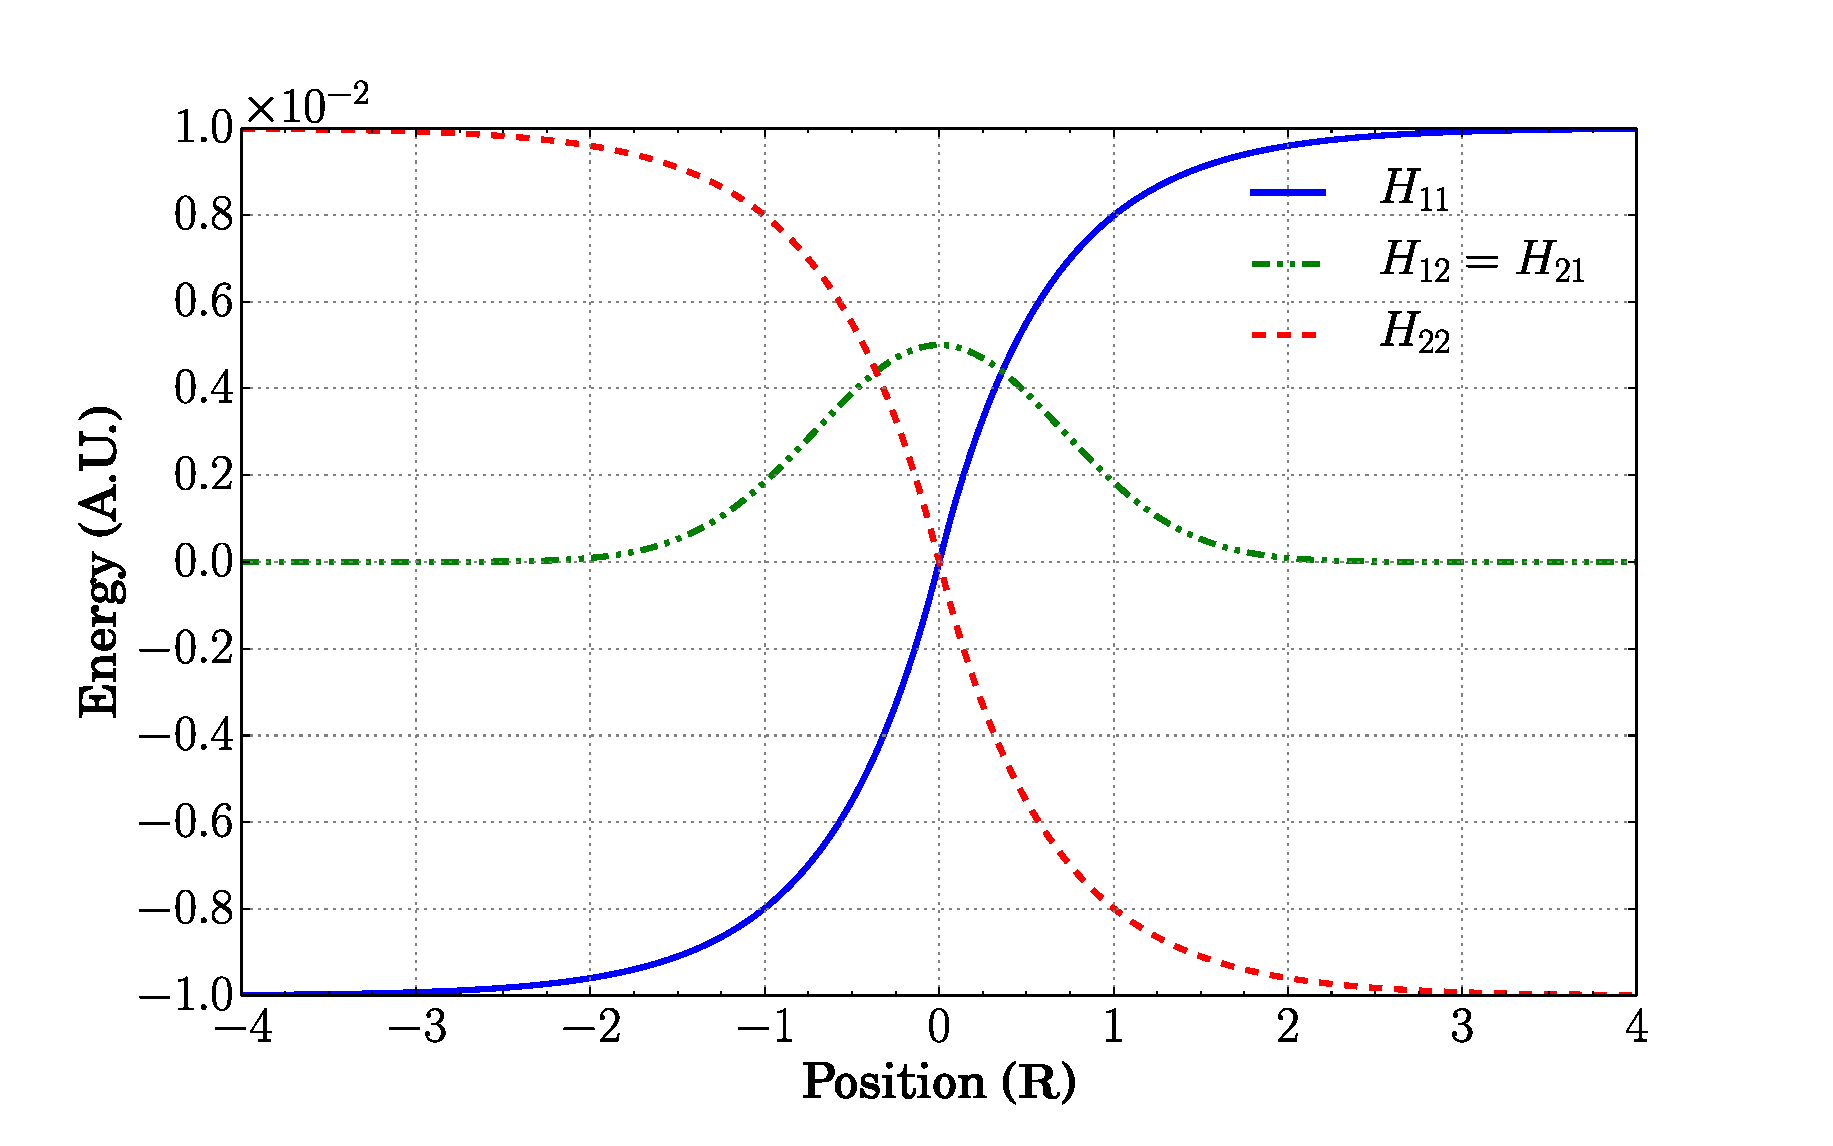
\includegraphics[width=\textwidth]{scpes.eps}
\caption[]{Diabatic PES.}
\label{sumf:pessc}
\end{subfigure}
~
\begin{subfigure}[t]{0.485\textwidth}
\centering
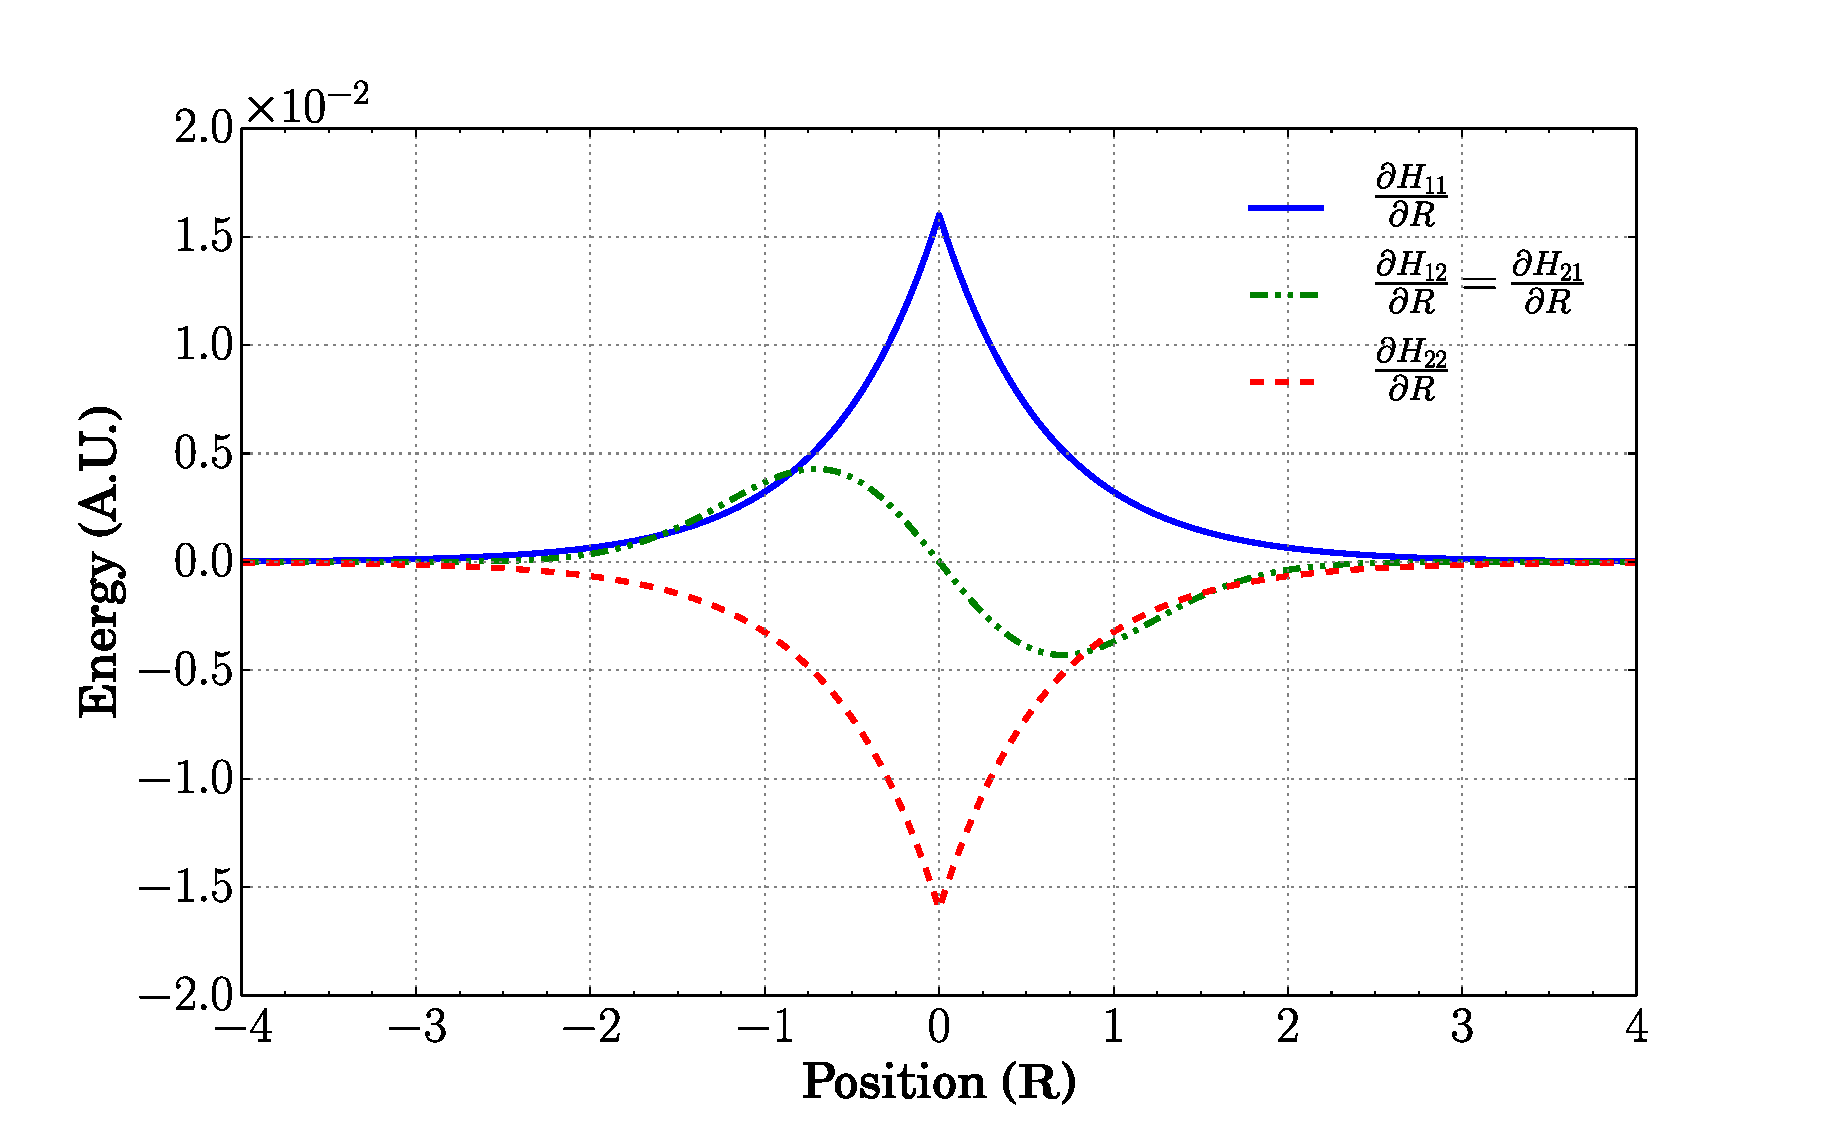
\includegraphics[width=\textwidth]{dscpes.eps}
\caption[]{Diabatic PES derivatives.}
\label{sumf:dpessc}
\end{subfigure}

\begin{subfigure}[t]{0.485\textwidth}
\centering
\includegraphics[width=\textwidth]{ascpes.eps}
\caption[]{Adiabatic PES.}
\label{sumf:apessc}
\end{subfigure}
~
\begin{subfigure}[t]{0.485\textwidth}
\centering
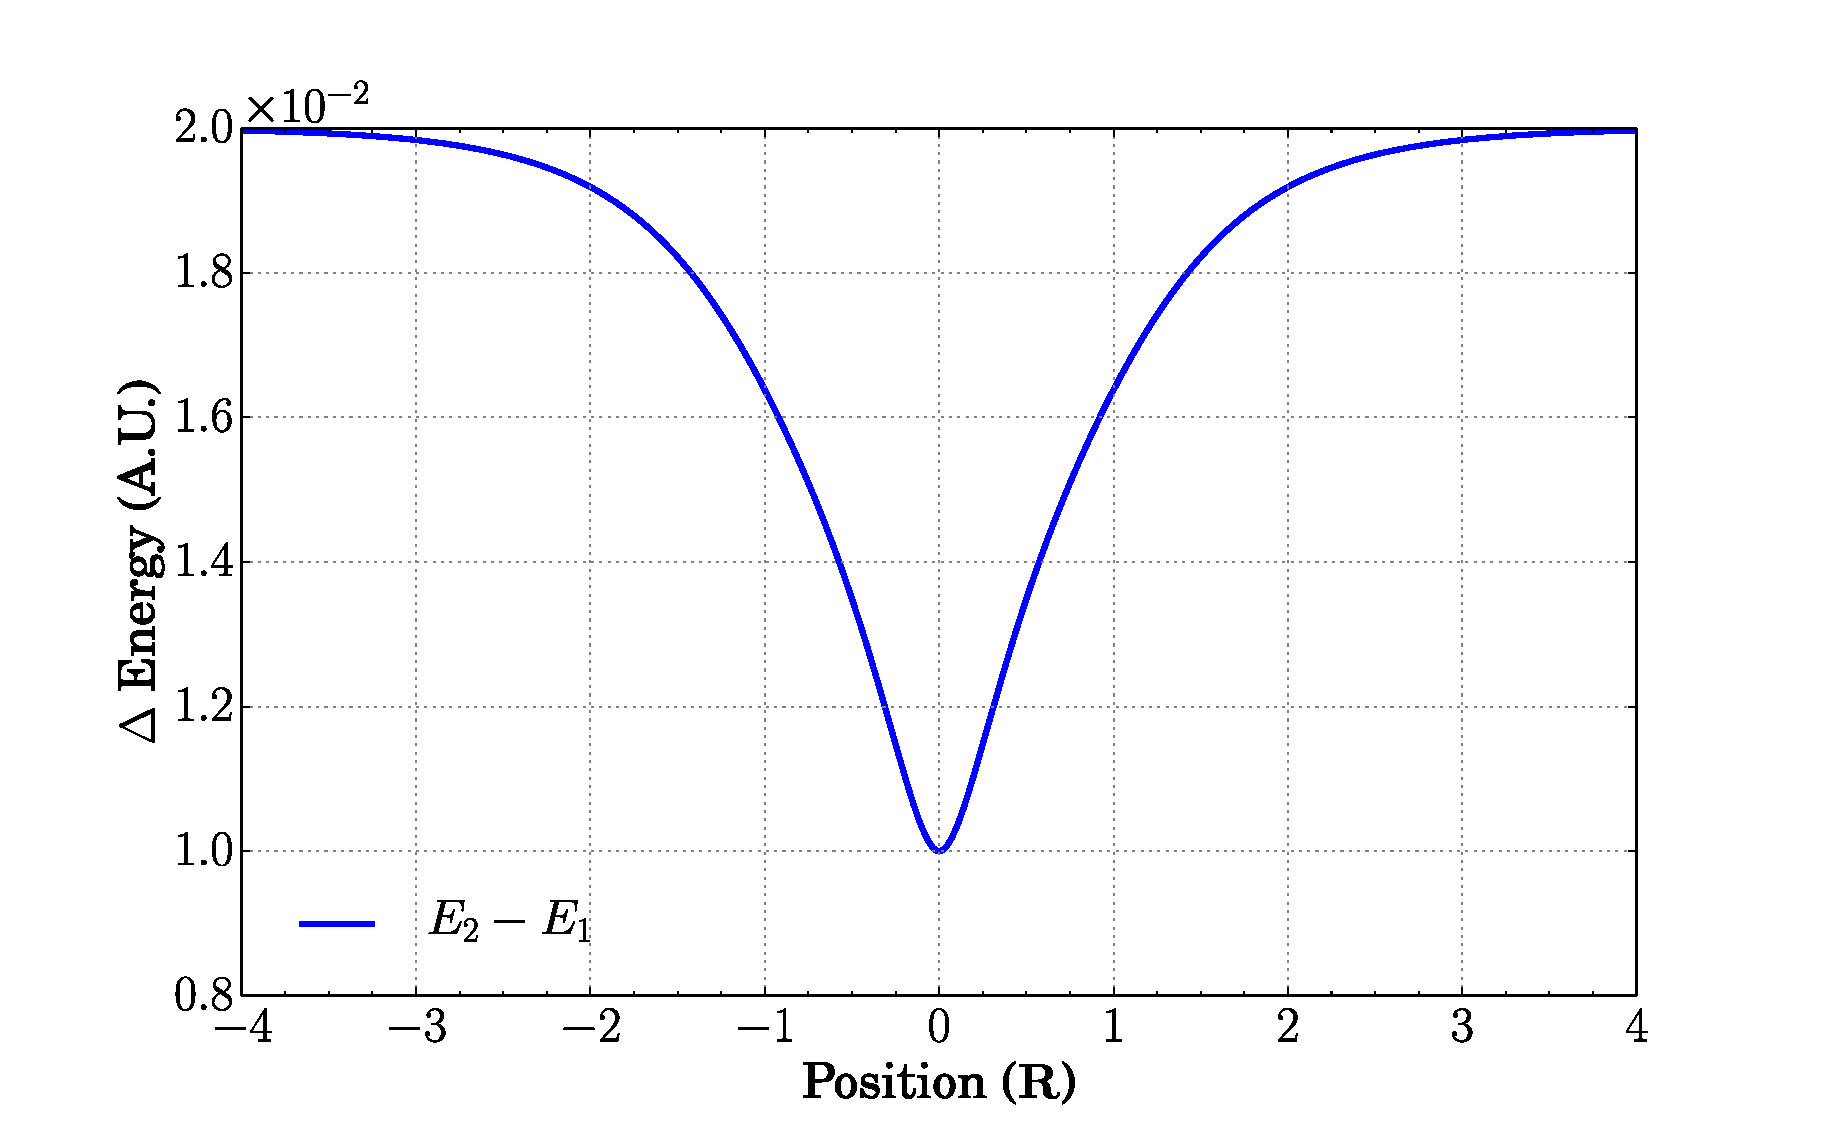
\includegraphics[width=\textwidth]{del_ascpes.eps}
\caption[]{$ \Delta E$ between adiabatic PES.}
\label{sumf:delapessc}
\end{subfigure}
\caption[]{Single avoided crossing PES.}\label{sumf:scpes}
\end{figure}
%
\subsection*{Double Avoided Crossing}
%
The diabatic potential energy surfaces (PES) for the double avoided crossing 
were defined by Tully \cite{tully} as:
\begin{subequations}
\begin{align}
H_{11}(R) &= 0 \\
H_{22}(R) &= -A e^{-B R^{2}} + E_{0}\\
H_{12}(R) &= H_{21}(R) = C e^{-D R^{2}}~,
\end{align}
\end{subequations}
where $ A = 0.1$, $B = 0.28$, $C = 0.015$, $D = 0.06$, y $E_{0} = 0.05$. The diabatic PES, their derivatives, adiabatic PES and $ \Delta E $ between adiabatic PES are plotted in \cref{sumf:dcpes}.

\begin{figure}
\centering
\begin{subfigure}[t]{0.485\textwidth}
\centering
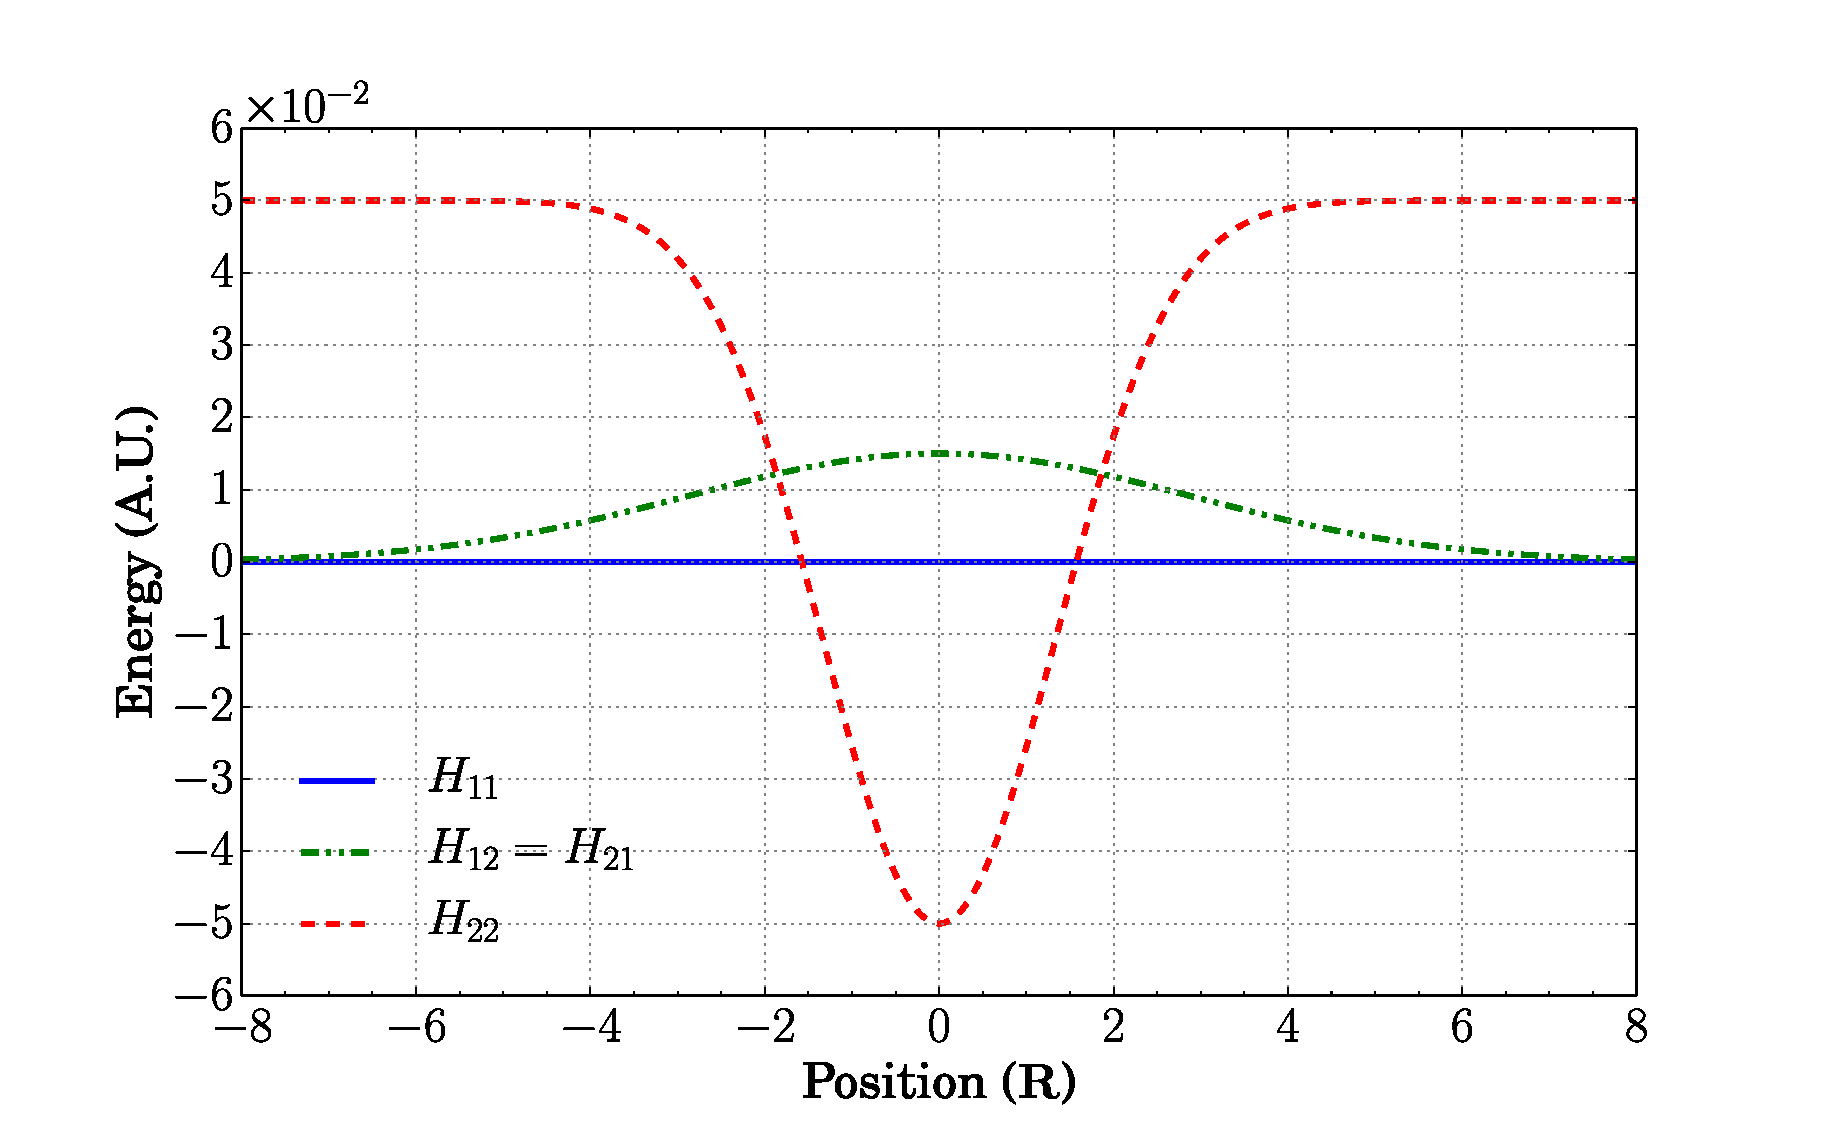
\includegraphics[width=\textwidth]{dcpes.eps}
\caption[]{Diabatic PES.}
\label{sumf:pesdc}
\end{subfigure}
~
\begin{subfigure}[t]{0.485\textwidth}
\centering
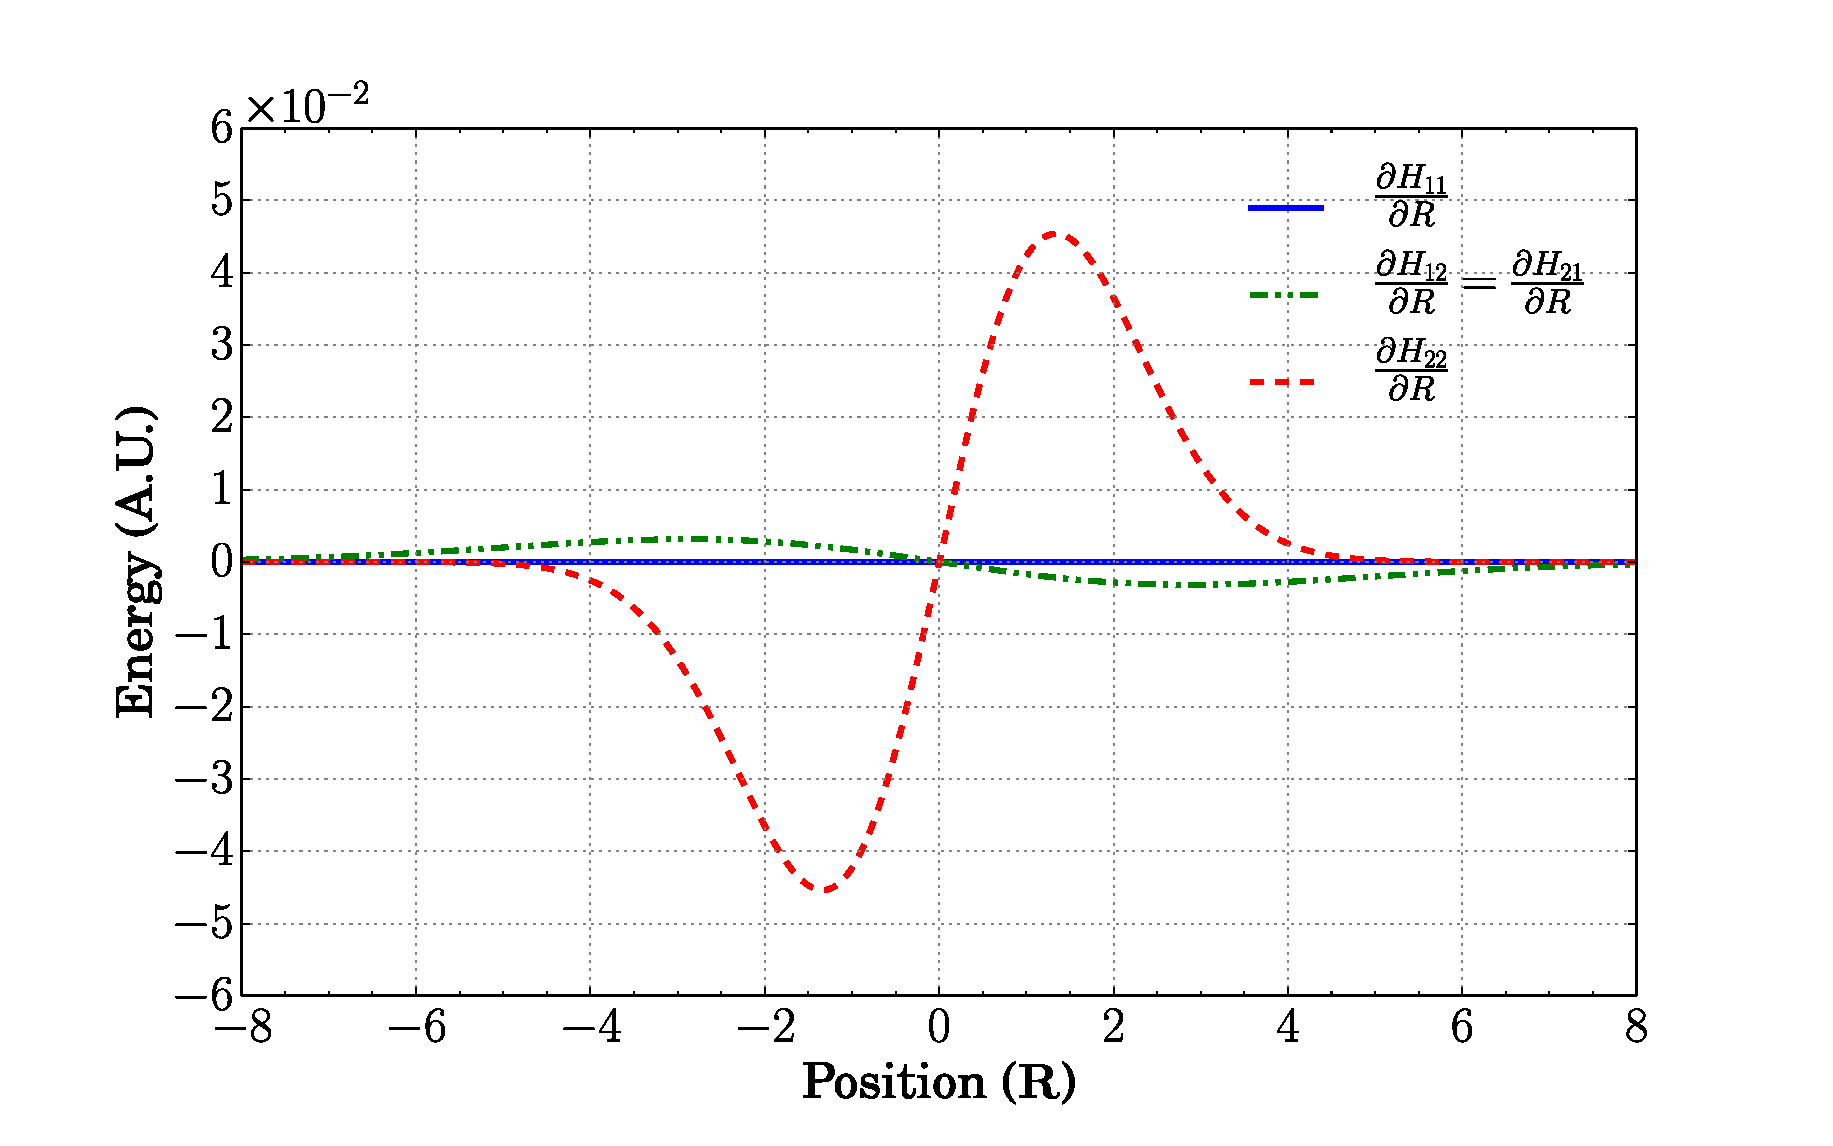
\includegraphics[width=\textwidth]{ddcpes.eps}
\caption[]{Diabatic PES Derivatives.}
\label{sumf:dpesdc}
\end{subfigure}

\begin{subfigure}[t]{0.485\textwidth}
\centering
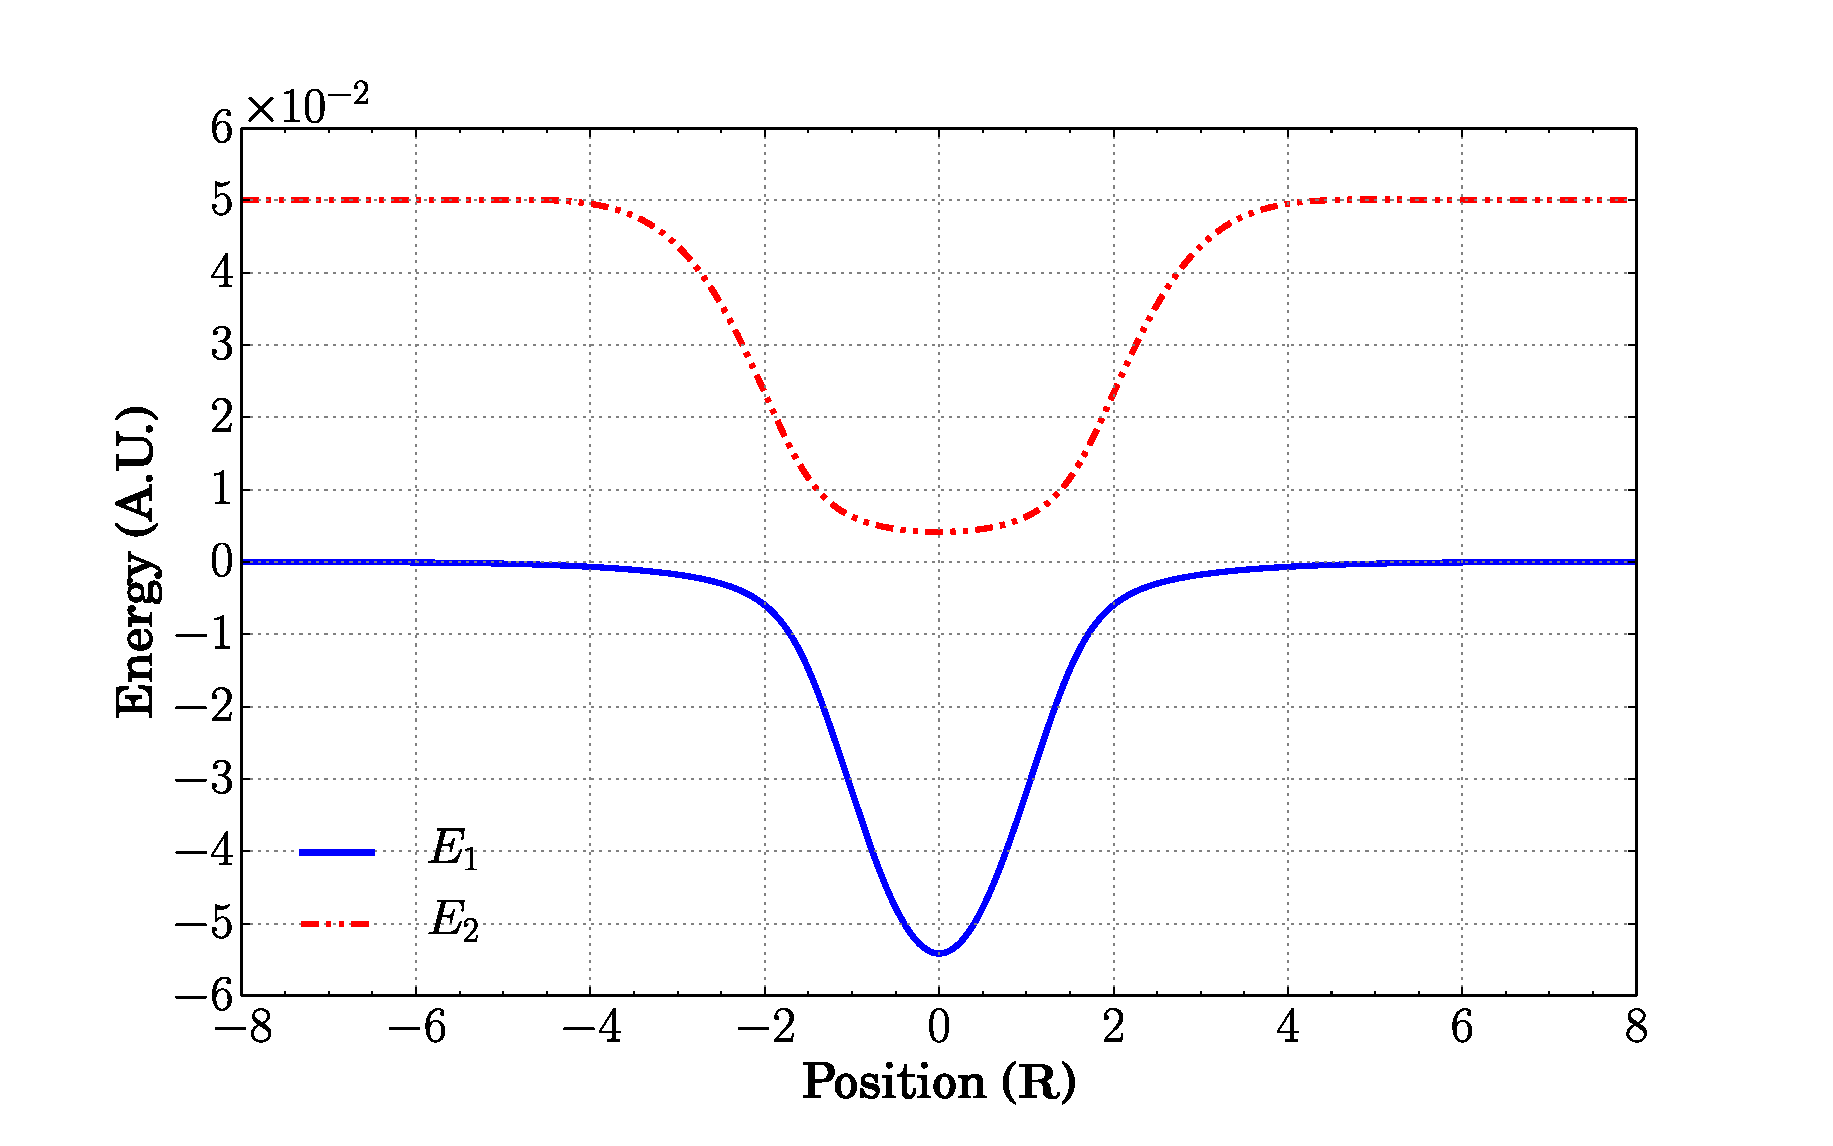
\includegraphics[width=\textwidth]{adcpes.eps}
\caption[]{Adiabatic PES.}
\label{sumf:apesdc}
\end{subfigure}
~
\begin{subfigure}[t]{0.485\textwidth}
\centering
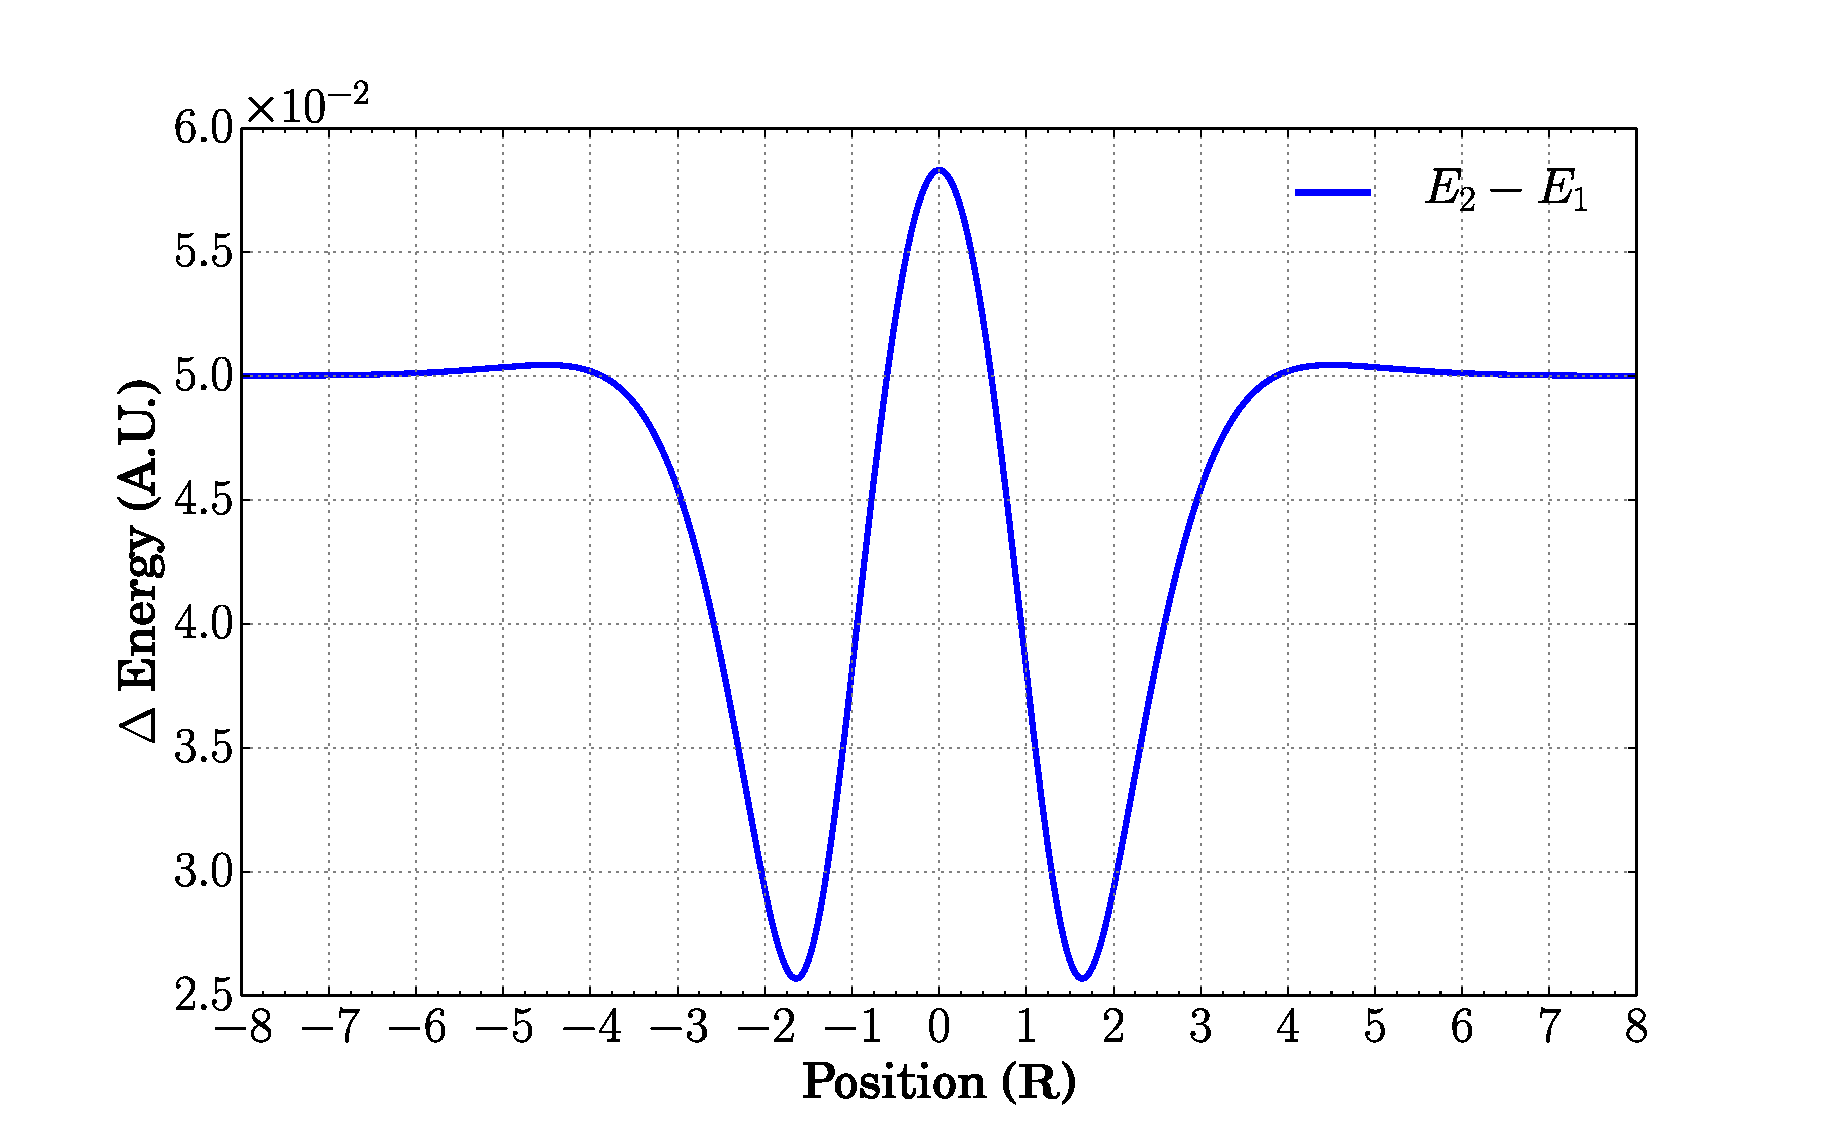
\includegraphics[width=\textwidth]{del_adcpes.eps}
\caption[]{$ \Delta E$ between adiabatic PES.}
\label{sumf:delapesdc}
\end{subfigure}
\caption[]{Double avoided crossing PES.}\label{sumf:dcpes}
\end{figure}
%
\subsection*{Extended Coupling}
%
The diabatic potential energy surfaces (PES) for the extended coupling 
were defined by Tully \cite{tully} as:
\begin{subequations}
\begin{align}
H_{11}(R) & = -A\\
H_{22}(R) & = -H_{11}\\
H_{12}(R) & = H_{21}(R) = 
\begin{cases}
B(2 - e^{-C R}) & R\geq 0 \\
B e^{C R} & R<0
\end{cases}
\end{align}
\end{subequations}
where $ A = 6 \times 10^{-4},~B = 0.1,~\text{and}~C = 0.9$. This problem has non-vanishing non-diagonal elements in the Hamiltonian matrix. Said elements are perturbations from a pure state, and when they do not vanish when $ R \rightarrow \pm\infty $, one must use the adiabatic Hamiltonian. \Cref{sumf:ecpes} shows the diabatic and adiabatic PES and their derivatives (the difference between both adiabatic PES is not shown because it's fairly obvious).

\begin{figure}
\centering
\begin{subfigure}[t]{0.485\textwidth}
\centering
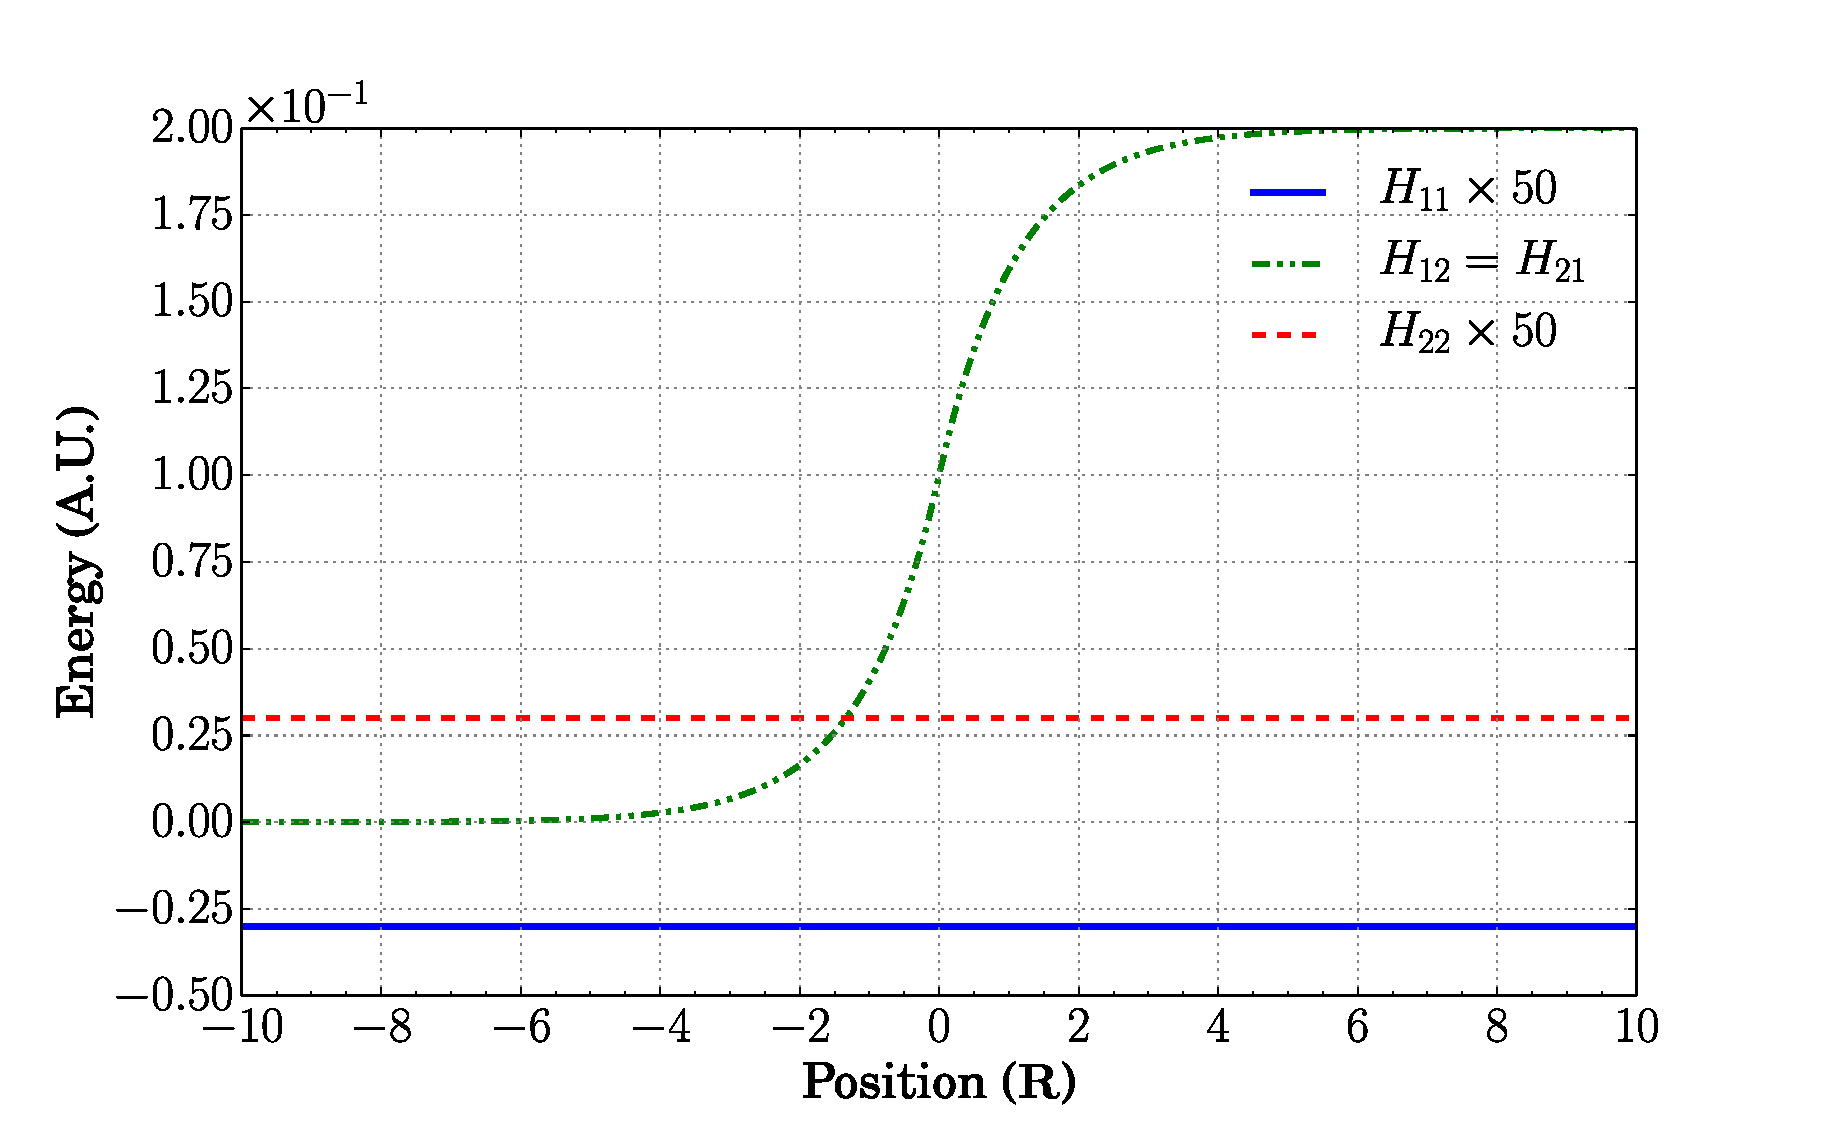
\includegraphics[width=\textwidth]{ecpes.eps}
\caption[]{Diabatic PES.}
\label{sumf:pesec}
\end{subfigure}
~
\begin{subfigure}[t]{0.485\textwidth}
\centering
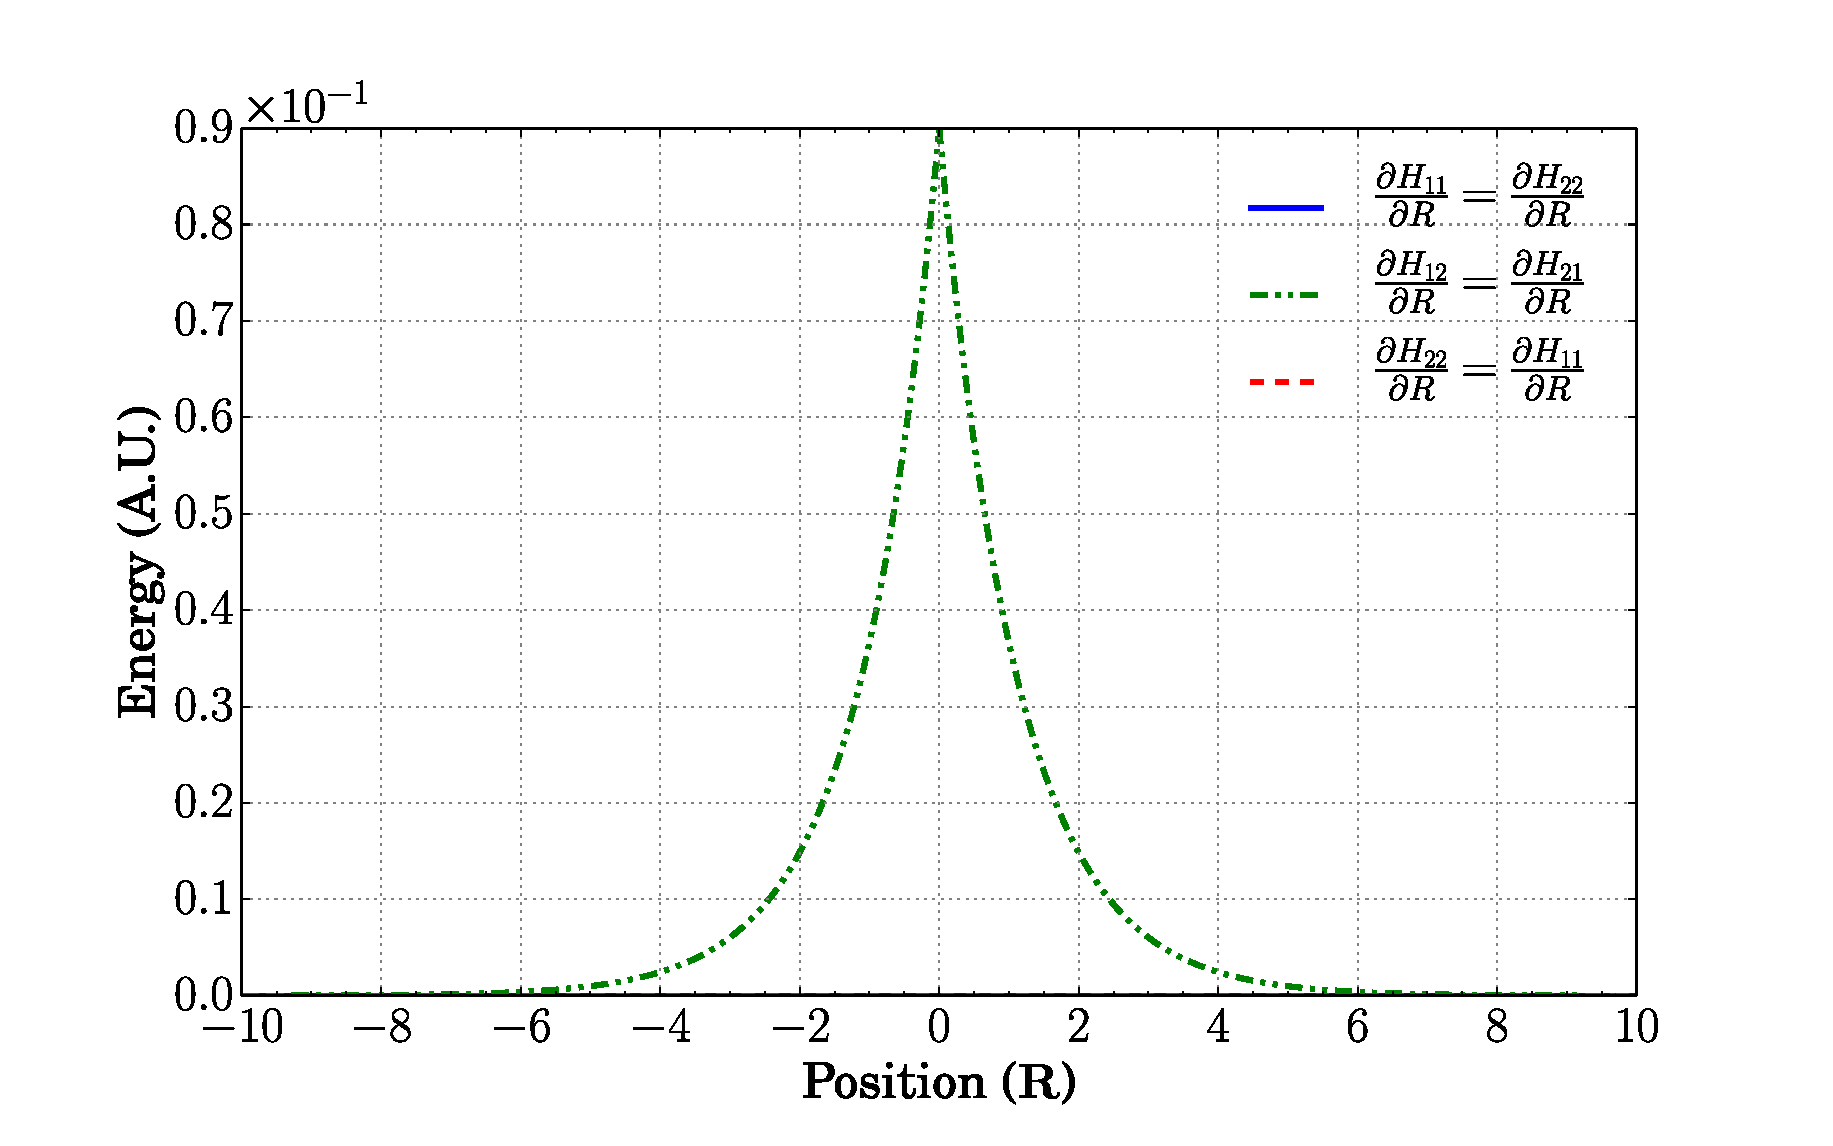
\includegraphics[width=\textwidth]{decpes.eps}
\caption[]{Diabatic PES derivatives.}
\label{sumf:dpesec}
\end{subfigure}

\begin{subfigure}[t]{0.485\textwidth}
\centering
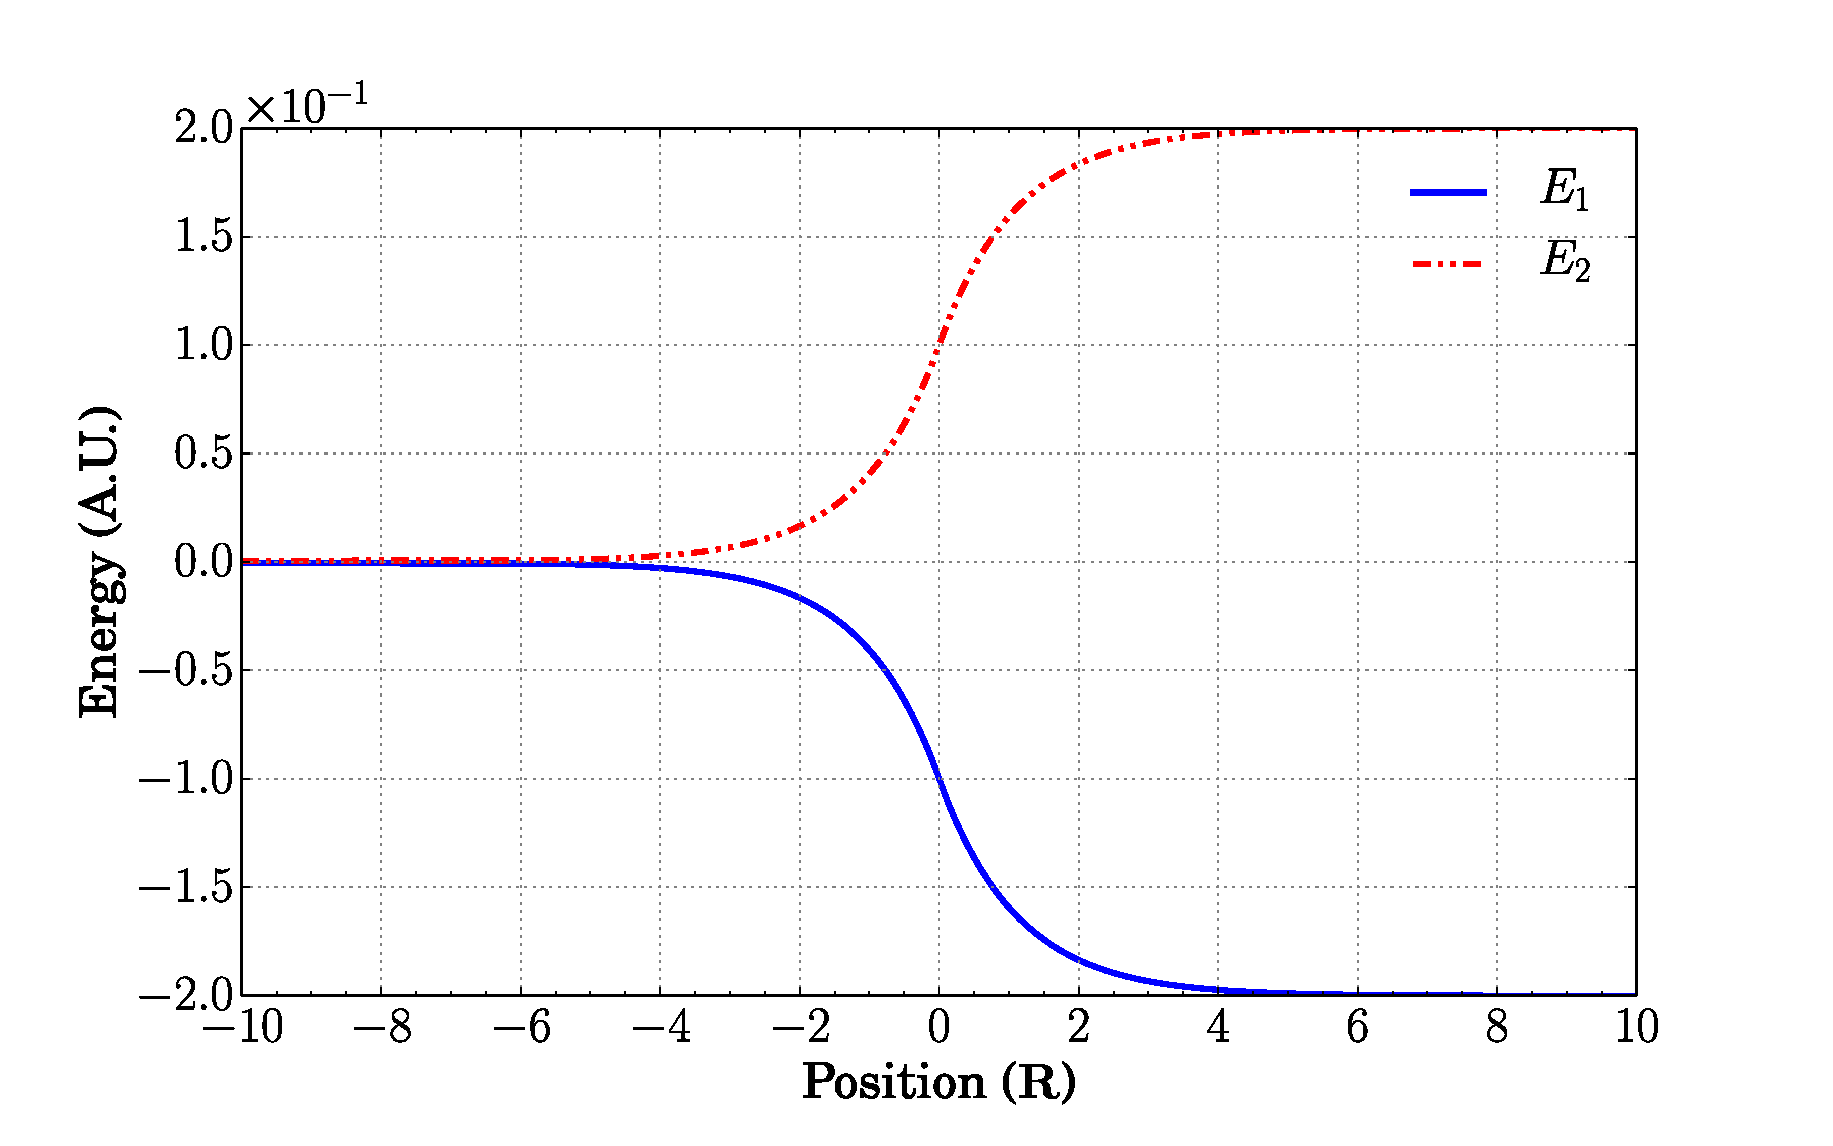
\includegraphics[width=\textwidth]{aecpes.eps}
\caption[]{Adiabatic PES.}
\label{sumf:apesec}
\end{subfigure}
~
\begin{subfigure}[t]{0.485\textwidth}
\centering
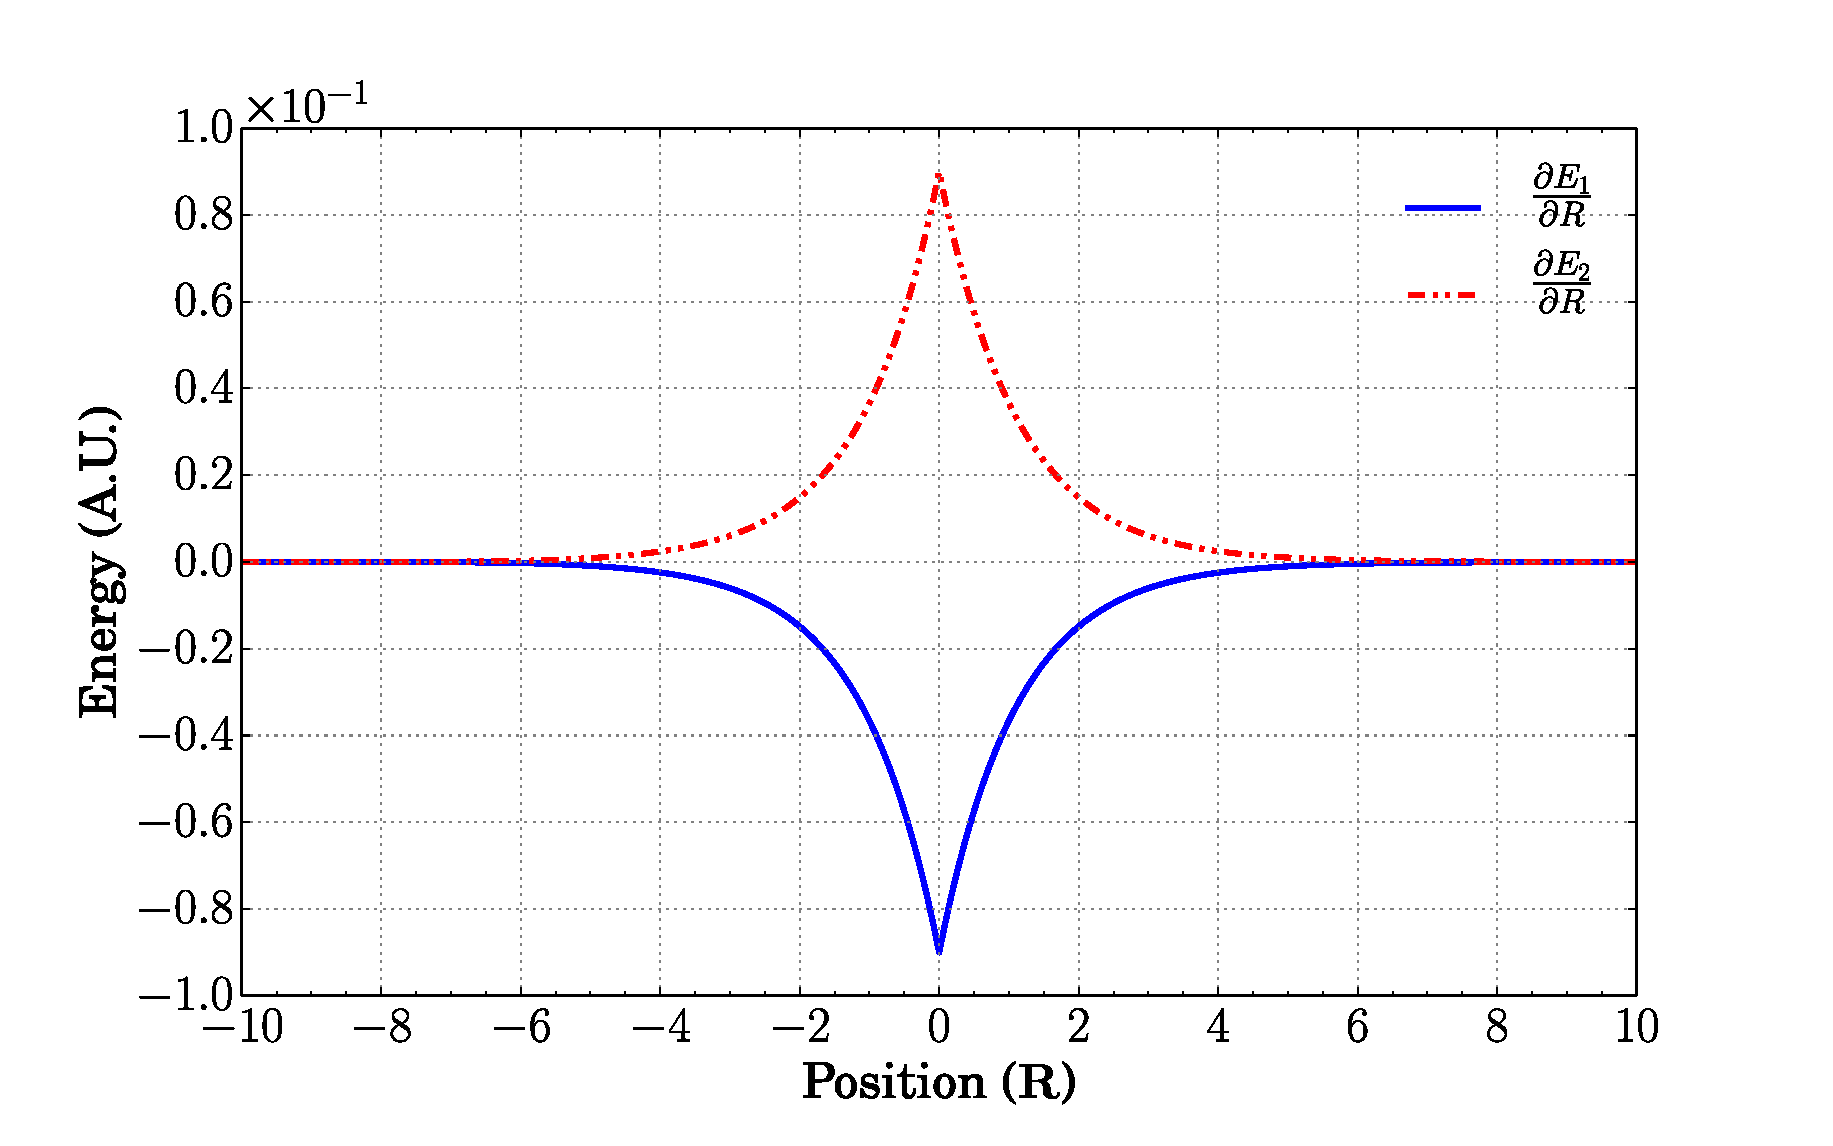
\includegraphics[width=\textwidth]{daecpes.eps}
\caption[]{Adiabatic PES derivatives.}
\label{sumf:dapesec}
\end{subfigure}
\caption[]{Extended coupling PES.}\label{sumf:ecpes}
\end{figure}
%
\subsection*{Spin-Boson Model for Condensed-Phase Dynamics}\label{sumsb:sb}
%
This problem is vastly different from the others. In our case, the model describes a 1D system of $ M $ coupled oscillators. More specifically, a one-dimensional lattice made up of $ M $ oscillating nuclei which posses bulk electronic states. What is measured here are not trajectories, but rather the time-dependent difference in the probability of finding the system in either of two electronic states; when the initial state $ =1 $, $ D(t) = P_{1\leftarrow 1} - P_{2\leftarrow 1}$, when the initial state $ =2 $, $ D(t) = P_{1\leftarrow 2} - P_{2\leftarrow 2}$.

The diabatic PES are defined as follows:
\begin{subequations}\label{e:sbpes}
\begin{align}
H_{11}(\bm{Q}) &= V_{0}(\bm{Q}) + V_{1}(\bm{Q}) + \epsilon \\
H_{22}(\bm{Q}) &= V_{0}(\bm{Q}) - V_{1}(\bm{Q}) - \epsilon \\
H_{12}(\bm{Q}) &= H_{12}(\bm{Q}) = \Delta~,
\end{align}
\end{subequations}
where,
\begin{subequations}
\begin{align}
V_{0}(\bm{Q}) &= \sum\limits_{k=1}^{M} \frac{1}{2} m_{k} \omega_{k}^{2} Q_{k}^{2} \\
V_{1}(\bm{Q}) &= \sum\limits_{k=1}^{M} c_{k} Q_{k}~.
\end{align}
\end{subequations}
For our purposes, the frequencies, $ \omega_{k} $, are uniformly distributed $ \in [0.01 \omega_{c},~4 \omega_{c}] $ \cite{spin-boson}, where $ \omega_{c} $ is known as the \emph{characteristic frequency}, and defines the system's overall time scale. The observant reader will realise this does not make a lot of sense on its own, because not all frequencies contribute to a system's energy in equal amounts. Which is why the coupling parameters, $ c_{k} $, are chosen so they obey the distribution:
\begin{align}\label{e:sb_dd}
J(\omega) = \frac{\pi}{2} \sum\limits_{k=1}^{M} \frac{c_{k}^{2}}{m_{k} \omega_{k}}  \delta(\omega - \omega_{k})~,
\end{align}
where $ J(\omega) $ is an Ohmic distribution defined as:
\begin{align}\label{e:sb_cd}
J(\omega) = \frac{\pi}{2} \alpha \omega \exp\left(-\frac{\omega}{\omega_{c}}\right)~,
\end{align}
where $ \alpha $ is the Kondo parameter (a coupling strength parameter). After equating \cref{e:sb_dd,e:sb_cd}, and integrating with respect to $ \omega $, we find the values of $ c_{k} $ to be:
\begin{subequations}
\begin{align}
c_{k} & = \sqrt{\frac{2}{\pi} \Delta \omega m_{k} \omega_{k} J(\omega_{k})}
= \omega_{k} \sqrt{\alpha \Delta \omega m_{k} \exp\left(-\frac{\omega_{k}}{\omega_{c}}\right)} \\
\Delta \omega &= \frac{\omega_{max} - \omega_{min}}{M - 1}~.
\end{align}
\end{subequations}

The initial electronic conditions are initiated in the same manner as before. However, the nuclear ones are not. As stated before, the model describes oscillating nuclei in a 1D lattice, and their momenta and positions are assumed to follow the Wigner distribution:
\begin{subequations}
\begin{align}
\rho(\bm{P},\bm{Q}) &= \prod\limits_{k=1}^{M} \exp\left(-a_{k} \frac{P_{k}^{2}}{2 m_{k}}\right)\cdot
\exp\left(-a_{k} \frac{1}{2} m_{k} \omega_{k}^{2} \left[Q_{k} + \frac{c_{k}}{m_{k} \omega_{k}^{2}}\right]^{2} \right)\\
a_{k} &= \frac{2}{\omega_{k}} \tanh\left(\frac{\beta \omega_{k}}{2}\right)~.
\end{align}
\end{subequations}
Which, in reality, is a bivariate normal distribution. Fortunately, the lack of a covariant term implies that positions and momenta can be independently sampled from normally distributed random numbers. In other words, the nuclei follow independent normal distributions for their momenta and positions. It is also worth noting that the argument for the total distribution is basically a scaled quasiclassical analogue of the quantum harmonic oscillator Hamiltonian operator ($ \hat{H} = \frac{\hat{p}^{2}}{2m} + \frac{1}{2} m \omega^{2} \hat{x}^{2}$), which makes a lot of intuitive sense, because it means the nuclear parameters are sampled according to the oscillators' normally distributed kinetic energy.

Sampling is done in the traditional way: assuming $ X $ is a normally distributed random number with unitary standard deviation and mean equal to zero, a normally distributed random number $ G $ with standard deviation equal to $ \sigma $ and mean equal to $ \mu $ can be calculated by $ G = \sigma X + \mu $. Given the definition of the normal distribution,
\begin{align}
G(x, \mu, \sigma) = \frac{1}{\sigma \sqrt{2\pi}} \exp\left(- \frac{(x-\mu)^{2}}{2 \sigma^{2}}\right),
\end{align}
the standard deviations and mean values of the nuclei's momenta and positions are:
\begin{subequations}
\begin{align}
&\sigma_{P_{k}} = \sqrt{\frac{m_{k} \omega_{k}}{2 \tanh\left(\frac{\beta \omega_{k}}{2}\right)}}\\
&\mu_{P_{k}} = 0\\
&\sigma_{Q_{k}} = \sqrt{\frac{1}{2 m_{k} \omega_{k} \tanh\left(\frac{\beta \omega_{k}}{2}\right)}}\\
&\mu_{Q_{k}} = -\frac{c_{k}}{m_{k} \omega_{k}^{2}}~.
\end{align}
\end{subequations}
%
\section*{Results}
%
The code written to implement the model was found to scale linearly with integration step, number of MC repetitions and number of cores used. It was also found that accuracy is more dependent on the number of MC repetitions than the size of the integration step, $ h $. In fact, the integration step could be made relatively large (how large depends on the problem) without significantly affecting accuracy, but drastically reducing computational time. There was also no significant difference between using $ \gamma = \frac{\sqrt{3}-1}{2} $ and $ \gamma = 0.366 $ (the actual value is very similar, but there is no need to evaluate square roots and divisions all the time if we use the approximation); \cite{project} gives the theoretical justification for this value, but it can be adjusted on a case by case basis. Accuracy was also not noticeably affected by parallel runs, presumably due to the random number generator used---which is thread safe---but not optimal for parallelisation, because it generates numbers in sequence from a single source rather than in parallel\footnote{See \url{https://gcc.gnu.org/onlinedocs/gfortran/RANDOM_005fNUMBER.html}} (it only affects execution speed).

The number of MC repetitions (MC reps) $ = 15000 $ and the value of $ \gamma = 0.366 $ unless stated otherwise. Reflections are denoted as $ R $ and transmissions as $ T $, electronic transitions from an initial state, $ i $, to a final state, $ f $, are denoted as $ f \leftarrow i $.
%
\subsection*{Single Avoided Crossing}
%
\begin{figure}
\begin{subfigure}[t]{0.5\textwidth}
\centering
\includegraphics[width=\textwidth]{sc_prob_lh.eps}
\caption[]{Transition probabilities for Reflection ($ R $) and Transmission ($ T $) for $ h = (0.012P_{i})^{-1} $ and initial state $ = 1 $.}
\label{sumf:sci1}
\end{subfigure}
~
\begin{subfigure}[t]{0.5\textwidth}
\centering
\includegraphics[width=\textwidth]{sc_prob_i2.eps}
\caption[]{Transition probabilities for Reflection ($ R $) and Transmission ($ T $) for $ h = (0.012P_{i})^{-1} $ and initial state $ = 2 $.}
\label{sumf:sci2}
\end{subfigure}
\caption[]{Single avoided crossing transition probabilities.}\label{sumf:sc}
\end{figure}

The results for when initial state $ = 1 $ are very similar---though not exactly the same---as those found in \cite{project}. However, this is most likely down to the fact that they used $ 50000\text{--}100000$ trajectories as well as there being a strong possibility that the compiler, RNG, and integration step differ. \Cref{sumf:sc} showcases the results for initial state $ = 1, 2 $.

Despite this being the simplest problem tackled herein, it presents some fairly interesting behaviours.

First, we shall tackle \cref{sumf:sci1}. The behaviour of \roo---whose probability is seen to rapidly decline as nuclear momentum increases---can be explained by referring back to \cref{sumf:scpes}. For small values of nuclear momentum, there is not enough kinetic energy to scale over the potential barrier (akin to an `activation energy') and continue in the original direction, thus the particle is reflected back. The behaviour of \rto~is explained by the same reason; once there is enough kinetic energy to reach a point where a transition is likely to happen, there would also be enough energy to continue on to the other side. Thus \rto~remains relatively close to zero throughout. The others can be explained by the fact that transition probabilities are not only a function of the distance between adiabatic PES, but also on the time it takes the particle to move away from the areas where this value is small. This explains why the \tto~and \too~transitions behave the way they do. In the case of \tto~lower nuclear momenta allow more time for an electronic transition to occur; however, after a certain value of nuclear momentum, it begins to decrease in favour of \too~because time the particle travels so fast that it cannot interact long enough to undergo an electronic transition.

For \cref{sumf:sci2} the behaviour is more nuanced, but down to mostly the same reasons. The \rot~transition remains effectively zero throughout because at such low values of nuclear momenta two things can happen: the particle can't get past the dip in $ E_{2} $ (if it doesn't move to the lower energy state) because it gets reflected back by the off-diagonal PES---corresponding to the \rtt~transition---or it moves down to the lower energy state, where the surplus potential energy is converted into kinetic energy (conservation of energy) and a \tot~transition is observed. For higher values of nuclear momentum, the particle has enough energy to be transmitted, but there is not enough time for the particle to linger long enough for there to be a state transition, and \ttt~is observed instead, and the higher the nuclear momentum the less time there is and the likelier said process becomes.
%
\subsection*{Double Avoided Crossing}
%
\begin{figure}
\begin{subfigure}[t]{0.5\textwidth}
\centering
\includegraphics[width=\textwidth]{dc_prob_lh.eps}
\caption[]{Transition probabilities for Reflection ($ R $) and Transmission ($ T $) for $ h = (0.0125P_{i})^{-1} $ and initial state $ = 1 $.}
\label{sumf:dci1}
\end{subfigure}
~
\begin{subfigure}[t]{0.5\textwidth}
\centering
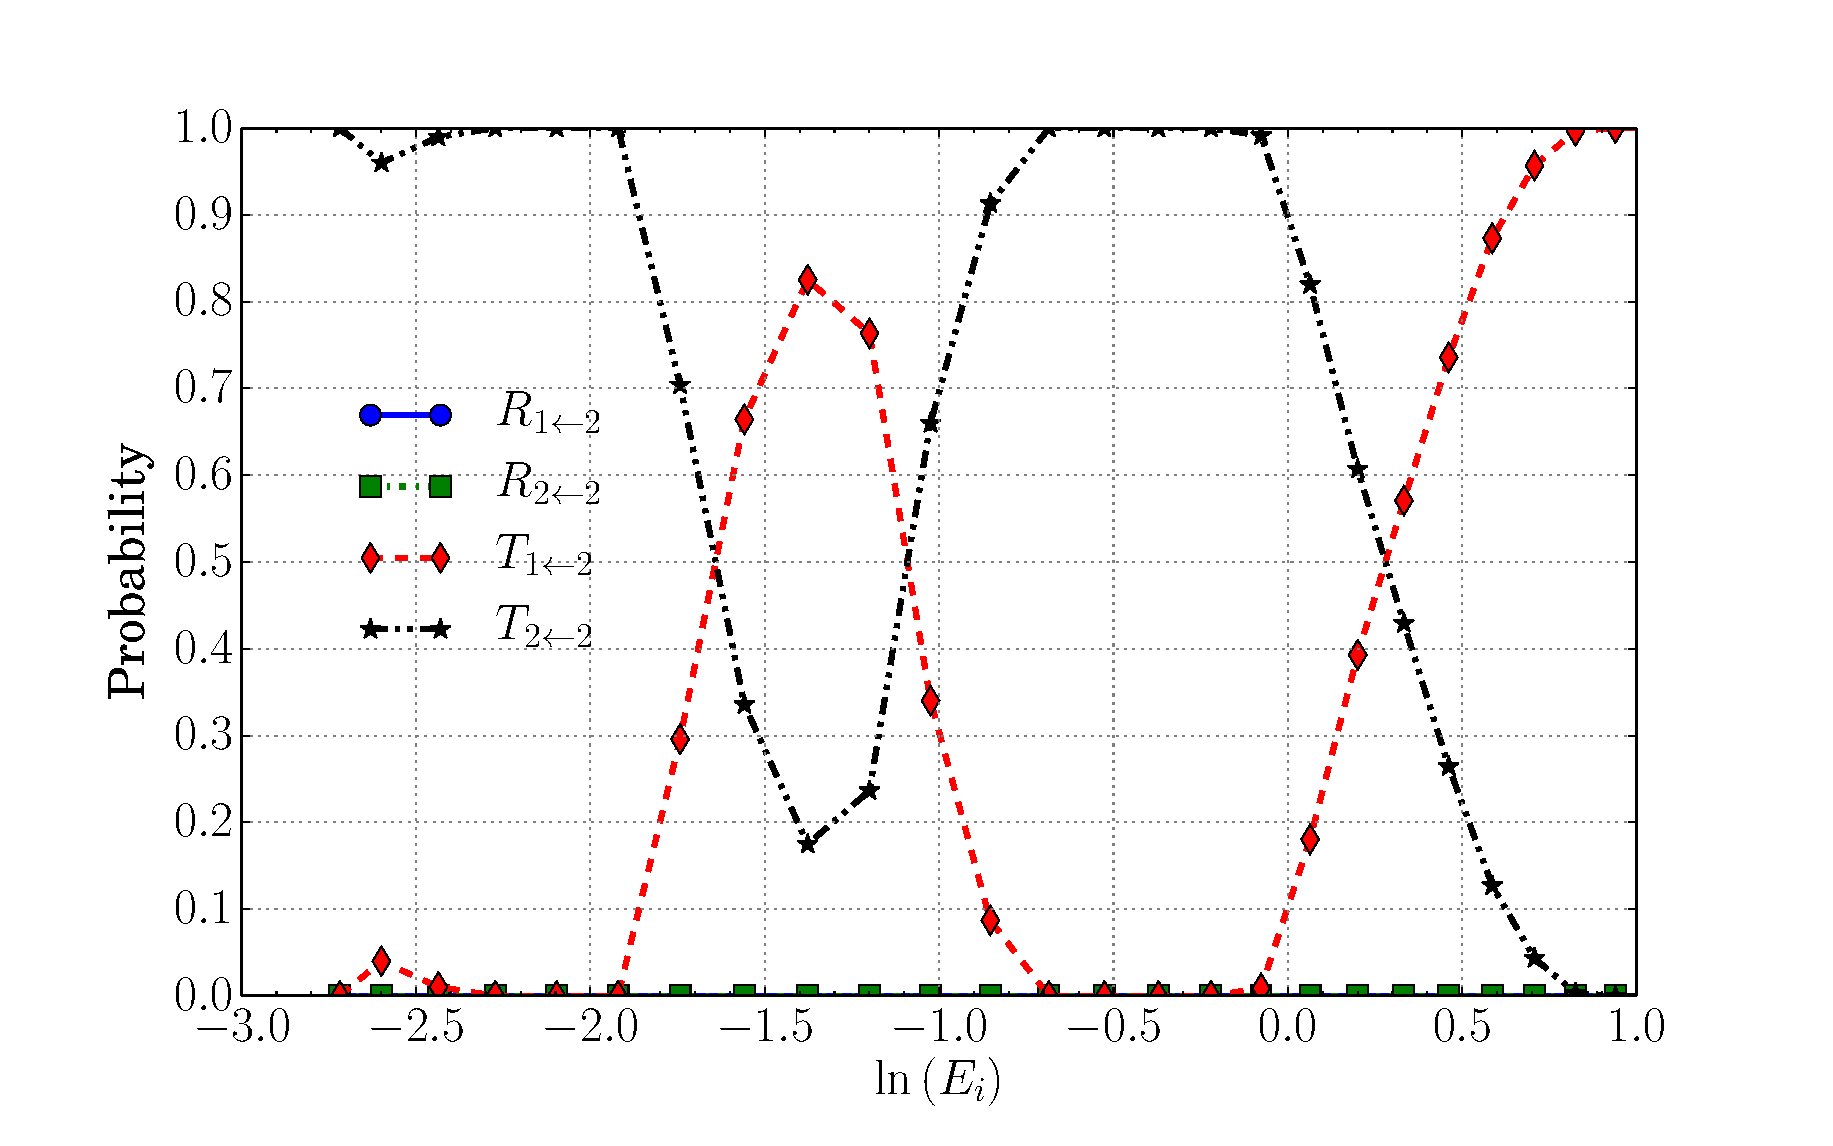
\includegraphics[width=\textwidth]{dc_prob_i2.eps}
\caption[]{Transition probabilities for Reflection ($ R $) and Transmission ($ T $) for $ h = (0.0125P_{i})^{-1} $ and initial state $ = 2 $.}
\label{sumf:dci2}
\end{subfigure}
\caption[]{Double avoided crossing transition probabilities.}\label{sumf:dc}
\end{figure}

Again the results for when initial state $ = 1 $ are very similar---but not exactly the same---as those found in \cite{project}. Which can be attributed to the same factors as before. \Cref{sumf:dc} shows the results for initial state $ = 1, 2 $.

Once more, we shall first analyse the behaviour for initial state $ = 1 $, shown in \cref{sumf:dci1}. The lack of \roo~and \rto~transitions is easily explained by the fact there is no energy barrier in either the diagonal diabatic or adiabatic PES (\cref{sumf:pesdc,sumf:apesdc}), therefore the particle only requires a small amount of momentum for the particle to be transmitted. In fact, in low momentum tests, the particle was accelerated by the adiabatic energy wells (potential energy was transferred into kinetic energy). The more interesting features are the Stückelberg oscillations for both \too~and \tto, which are often attributed to quantum interference effects. In order to comprehend these one must only turn to \cref{sumf:delapesdc}, which shows the difference between adiabatic PES. One can see that $ E_{2} - E_{1} $ varies quickly and by relatively large amounts, causing the system's electronic coordinates to vary wildly and quickly. For small momenta, the particle generally does not have enough energy to switch electronic states, leading to the relatively flat appearance of both \too~and \tto~from $ -4~\text{to}~-2 $. However, as momentum increases, there is enough energy to make one jump but not a lot to make the second one, leading to the behaviour seen from $ -2~\text{to}~-1 $. As momentum keeps increasing, there is enough energy for the second jump, and we get the behaviour we see from $ -1~\text{to}~0 $. Finally, when momentum is very large, the particle carries out one transition but does not linger long enough to make a second, leading to the behaviour we see from $ 0~\text{to}~1 $.

When the initial state $ = 2 $ (\cref{sumf:dci2}), the behaviour is very similar but inverted to the one described in the previous paragraph. In other words, the transmission which preserves the initial state, \ttt~in \cref{sumf:dci2}, is very similar in shape to the transmission which preserves the initial state, \too~in \cref{sumf:dci1}. And the transmission which does not preserve the initial state, \tot~in \cref{sumf:dci2}, is also very qualitatively similar to the transition which does not preserve the initial state, \tto~in \cref{sumf:dci1}. Which means they have similar explanations, with only the exact points at which these `domains' appear, varying between both initial states.
%
\subsection*{Extended Coupling}
%
\begin{figure}
\begin{subfigure}[t]{0.5\textwidth}
\centering
\includegraphics[width=\textwidth]{ec_prob_lh_mean.eps}
\caption[]{Transition probabilities for Reflection ($ R $) and Transmission ($ T $) for $ h = (0.10125 P_{i})^{-1} $, $ 30000 $ MC reps, and initial state $ = 1 $.}
\label{sumf:eci1}
\end{subfigure}
~
\begin{subfigure}[t]{0.5\textwidth}
\centering
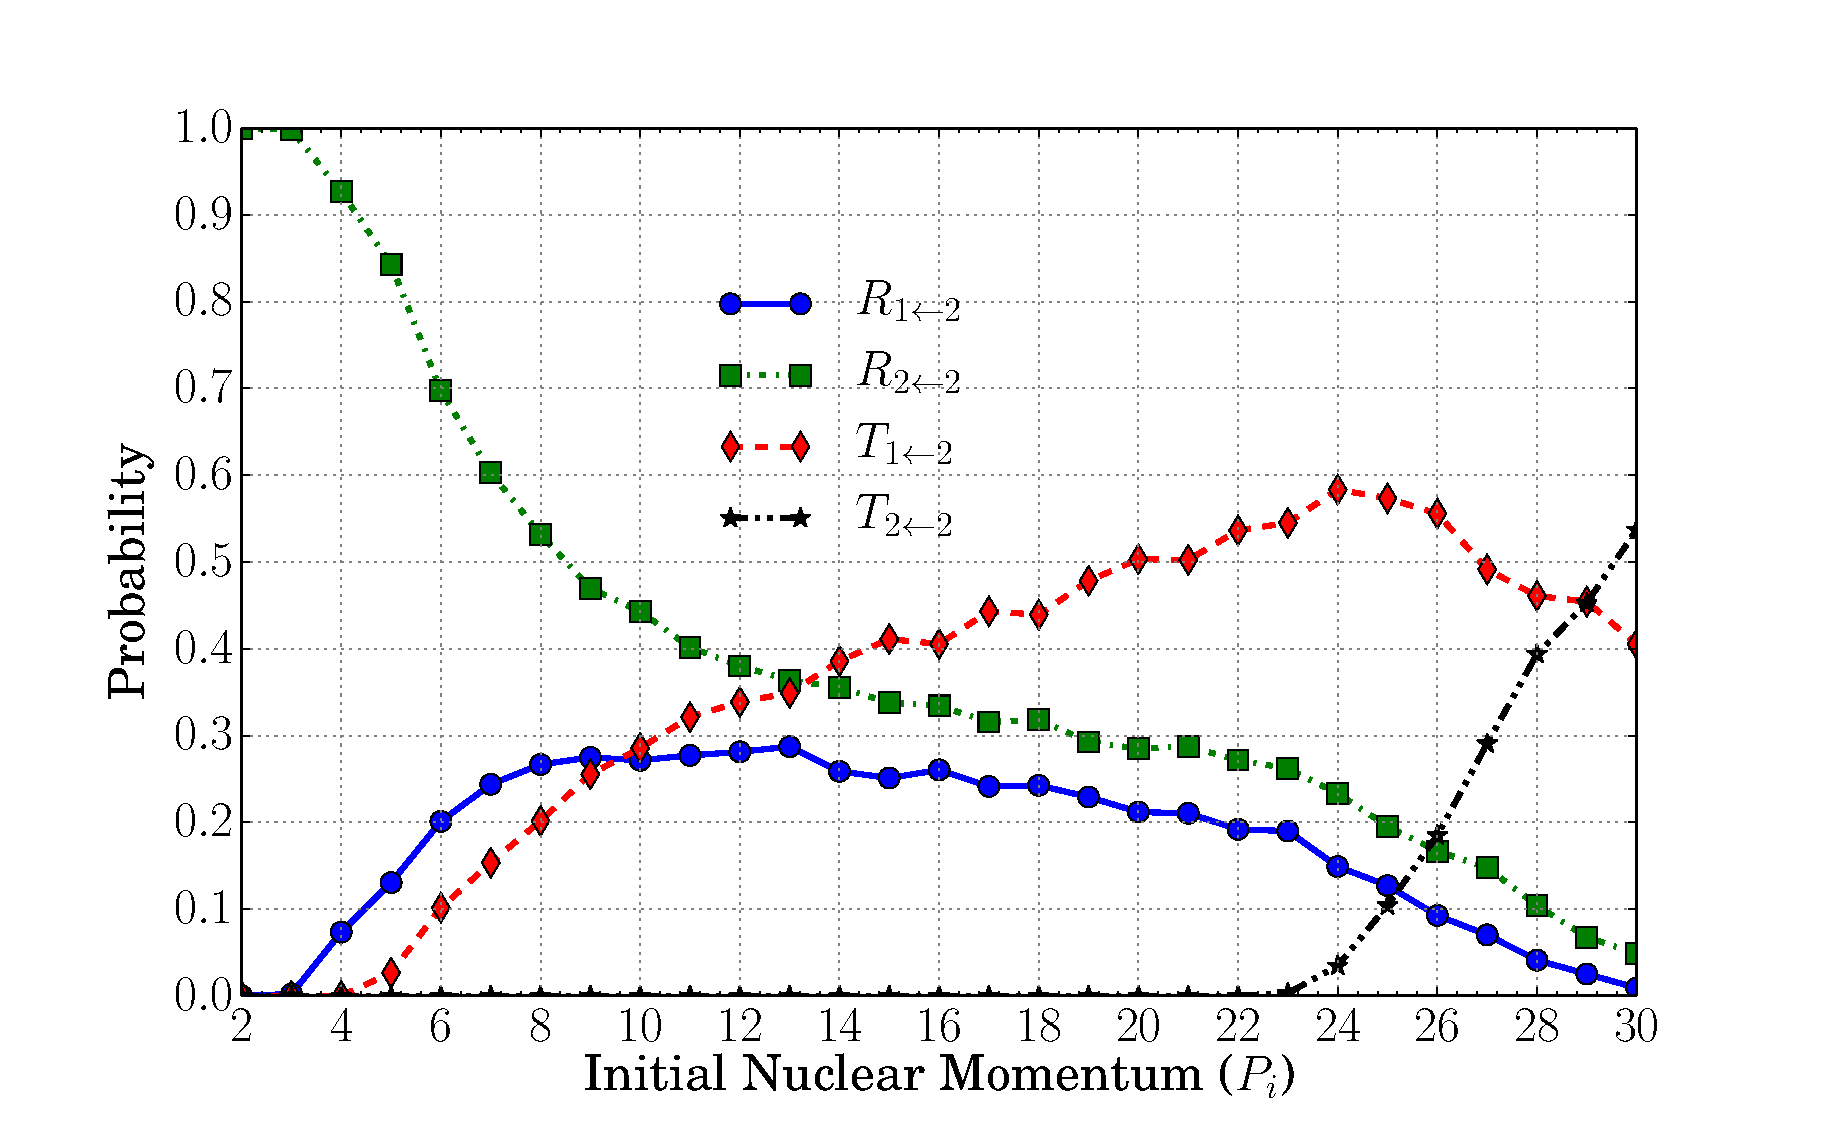
\includegraphics[width=\textwidth]{ec_prob_i2.eps}
\caption[]{Transition probabilities for Reflection ($ R $) and Transmission ($ T $) for $ h = (0.10125 P_{i})^{-1} $ and initial state $ = 2 $.}
\label{sumf:eci2}
\end{subfigure}
\caption[]{Extend coupling transmission probabilities.}\label{sumf:ec}
\end{figure}

Once more, the results for when initial state $ = 1 $ are very similar---but not exactly the same---as those found in \cite{project}. Which can again be attributed to the same factors as before. \Cref{sumf:ec} shows the results for initial states $ = 1, 2 $.

Following previously set precedents, we shall start the analysis with \cref{sumf:eci1} for which initial state $  = 1 $. The behaviour of \too~at low momenta is due to the fact that $ E_{1} $ is highly attractive, so the particle is easily transmitted without strongly interacting with any other PES. However, as the momentum increases the particle starts interacting more strongly with the non-diagonal elements of the hamiltonian matrix, $ H_{12} $, and it becomes more likely to either be reflected by it with or without an electronic transition, giving rise to the bump in probability of \roo~and \rto, and the dip in the probability of \too. It is only at higher nuclear momenta that it is possible for the particle to experience an electronic transition and have enough momentum to work against the repulsive interaction with and $ E_{2} $, leading to a probability increase of \tto.

For the case when the initial state $ = 2 $ (\cref{sumf:eci2}), the system's behaviour changes drastically. At low nuclear momenta, the particle does not have the required energy to be transmitted or undergo an electronic transition, leading to the shape of \rtt. However, as the momentum increases, the particle starts being able to change electronic state and be transmitted, leading to the increase in the probabilities of \rot~and \tot. As the momentum is increased further, the probability of having enough energy to transition into the lower electronic state and be transmitted increases, leading to the drop in \rtt~and \rot, and increase of \tot. As the nuclear momentum increases further, then the particle is travelling fast enough that it can overcome the repulsive effect of $ E_{2} $ and interact relatively little with $ E_{1} $, leading to the increased probability of observing \ttt.
%
\subsection*{Spin-Boson Model for Condensed-Phase Dynamics}
%
\begin{figure}
\begin{subfigure}[t]{0.5\textwidth}
\centering
\includegraphics[width=\textwidth]{spin_boson_e11.eps}
\caption[]{Initial state $ = 1$. For both systems $ h = 0.01$.}
\label{sumf:sbe11}
\end{subfigure}
~
\begin{subfigure}[t]{0.5\textwidth}
\centering
\includegraphics[width=\textwidth]{spin_boson_e12.eps}
\caption[]{Initial state $ = 2 $. For the symmetric problem, $ h = 0.1 $ and MC reps $ = 5000 $. For the asymmetric problem, $ h = 0.01 $ and MC reps $ = 30000 $.}
\label{sumf:sbe12}
\end{subfigure}
\caption[]{Spin-boson calculations for symmetric ($ \epsilon = 0 $) and asymmetric ($ \epsilon = 1 $) systems. $\alpha = 0.09,~\beta = 0.25,~\Delta = (2.5)^{-1}$.}\label{sumf:sb1}
\end{figure}

Some details were left out of \cite{project} in regards to this problem---namely the value of $ \omega_{c} $, and the range and distribution of $ \omega_{k} $---so it was assumed that $ \omega_{c} = 1$ and $ \omega_{k} $ uniformly distributed $\in [0.01\omega_{c},~4\omega_{c}] $ \cite{spin-boson}, and everything else was defined from there; which means there is no standard with which to compare results. \Cref{sumf:sb1,sumf:sb2} show the results of four systems (two symmetric and two asymmetric) characterised by different parameters, for initial electronic states $ = 1, 2 $. The calculations were carried out for 100 nuclei ($ M=100 $).

\Cref{sumf:sb1} shows incoherent (non-oscillatory) relaxation dynamics for all four systems. It is particularly interesting how much the behaviour changes between the symmetric and asymmetric version of each problem. In both cases, the asymmetric system favours the second state. Which means that the second state has a lower energy than the first. This notion is also evidenced by the fact that both symmetric systems stabilise at negative values of $ D(t) $, signifying that the probability of finding the system in state 2 is higher than that of finding it in state 1. This can potentially be observed from \cref{e:sbpes}.

On the other hand, \cref{sumf:sb2} shows both, coherent (oscillatory) and incoherent (non-oscillatory) relaxation dynamics. For both initial states, the symmetric system manifests highly oscillatory behaviours. But the surprising results arise from their asymmetric counterparts. Such results mean that for our chosen parameters, the dynamical system described by the equations of motion has large regions of stability in the electronic phase space. Such phenomena are not unheard of---where the same equations with different parameters yield vastly different results, ranging from nicely behaved to chaotic systems. Suffice to say, this was completely unexpected (and probably highly coincidental).

\begin{figure}
\begin{subfigure}[t]{0.5\textwidth}
\centering
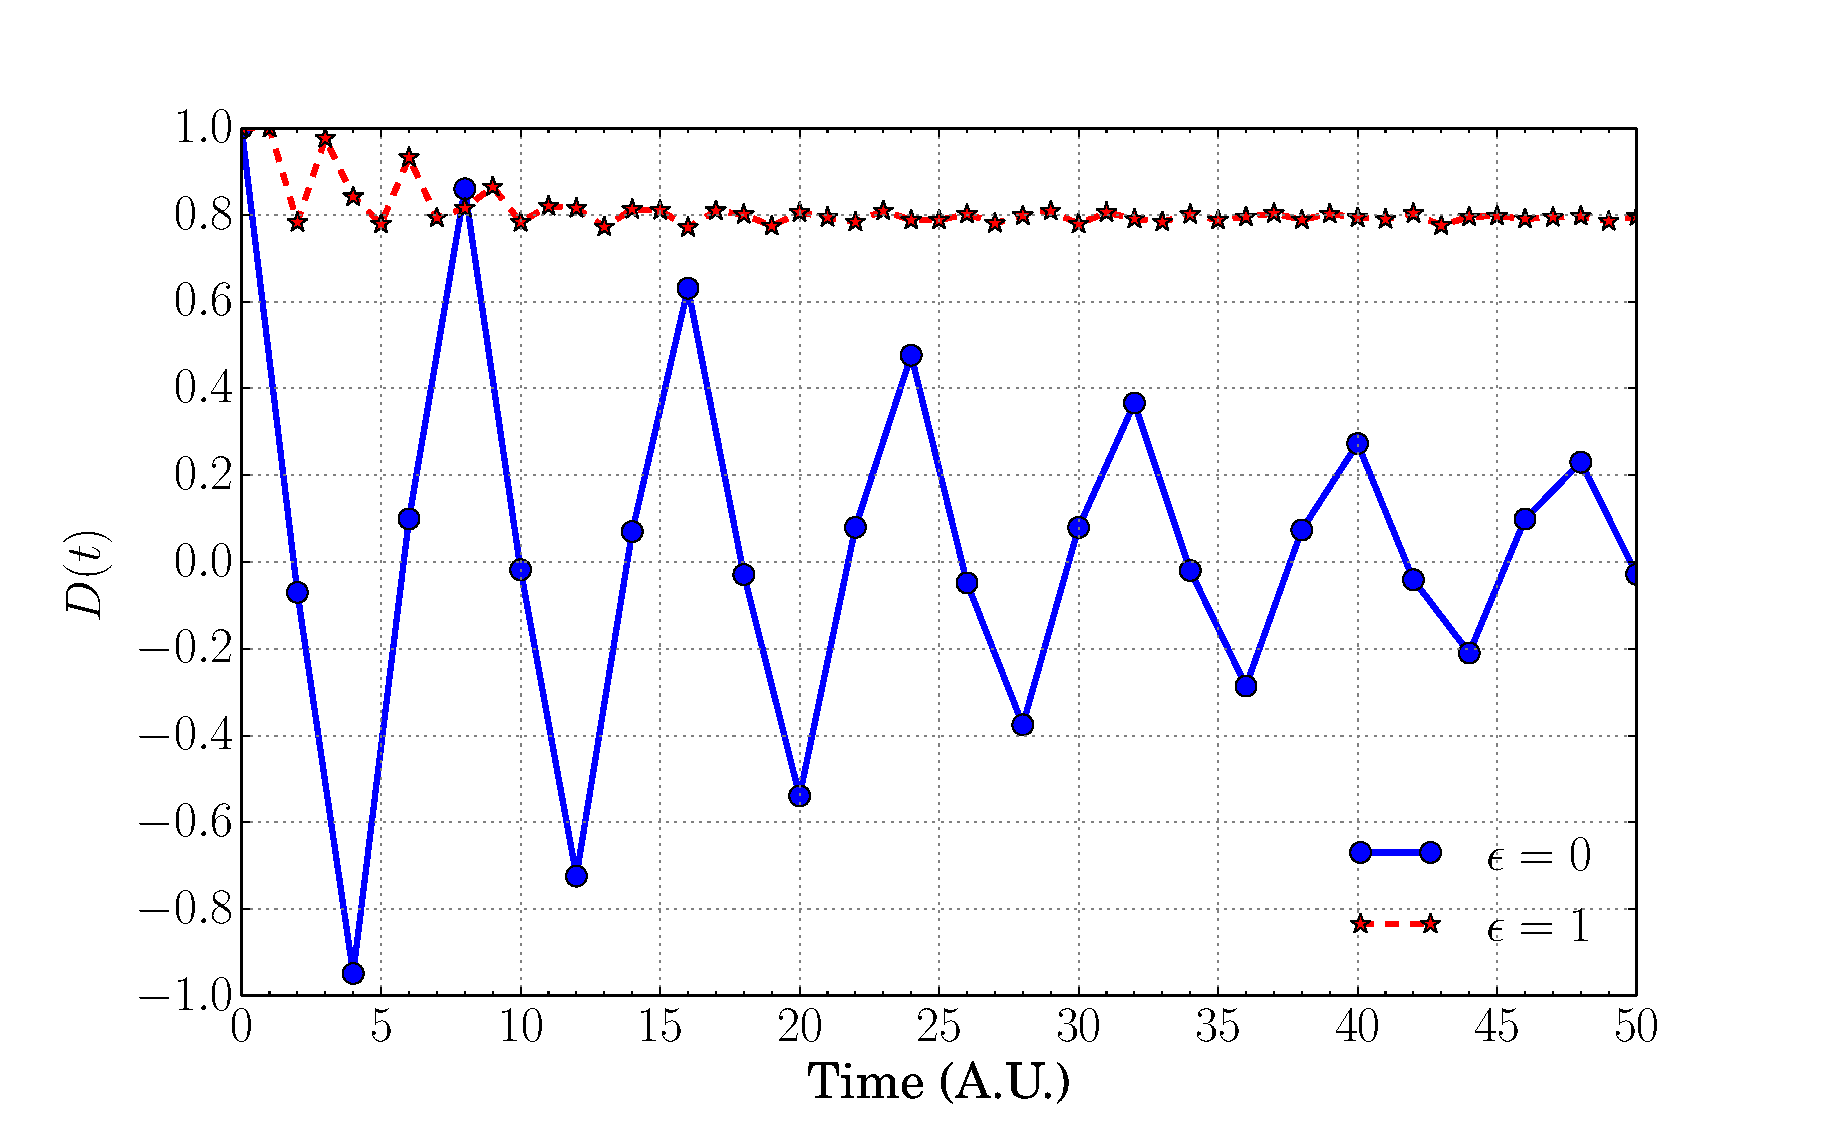
\includegraphics[width=\textwidth]{spin_boson_e21.eps}
\caption[]{Initial state $ =1 $. For the symmetric problem, $ h = 0.1 $ and MC reps $ = 5000 $. For the asymmetric problem, $ h = 0.05 $ and MC reps $ = 30000 $.}
\label{sumf:sbe21}
\end{subfigure}
~
\begin{subfigure}[t]{0.5\textwidth}
\centering
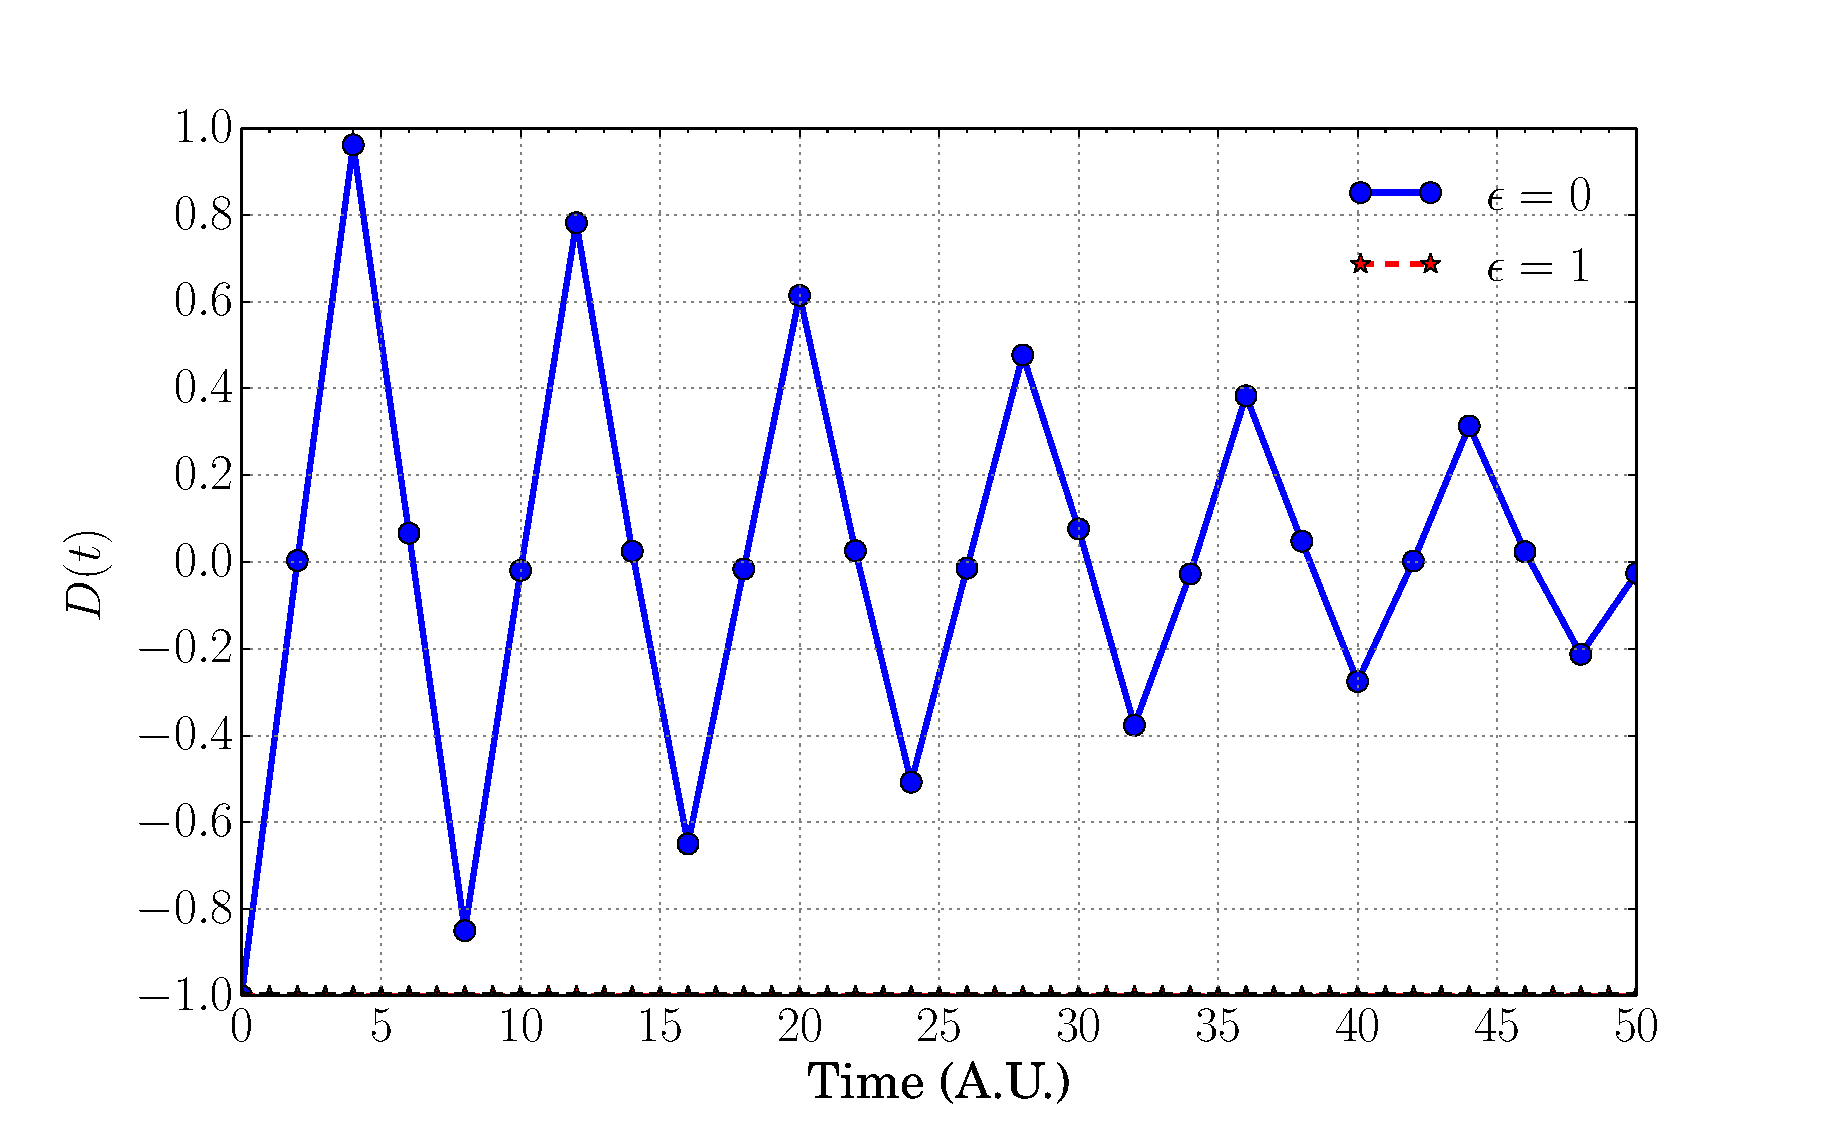
\includegraphics[width=\textwidth]{spin_boson_e22.eps}
\caption[]{Initial state $ = 2 $. For the symmetric problem, $ h = 0.1 $ and MC reps $ = 5000 $. For the asymmetric problem, $ h = 0.05 $ and MC reps $ = 30000 $.}
\label{sumf:sbe22}
\end{subfigure}
\caption[]{Spin-boson calculations for symmetric ($ \epsilon = 0 $) and asymmetric ($ \epsilon = 1 $) systems. $\alpha = 0.1,~\beta = 12.5,~\Delta = (2.5)^{-1}$.}\label{sumf:sb2}
\end{figure}

To conclude with this discussion, it must be said that the disparity in integration step and MC reps is down to each individual system's run time. The aforementioned quantities were adjusted so that no run exceeded 17 hours. There was some overcompensation in a few systems due to the highly variable nature of their run times, which in one instance was observed to exceed $ 250000\% $, though less extreme examples fell in the range of $ 300\%~\text{to}~1000\% $. This phenomenon is attributed to the large number of uniformly and normally distributed random numbers required to set the initial conditions---given that some of them do not allow the selection criteria to be met. The problem was compounded by the random seed allocation at every MC rep, and by the fact that the selection criteria (\cref{e:select}) must be met at every plot point, otherwise the MC rep has to be restarted.
%
\section*{Conclusions}
%
The most recent version of the MM model was successfully implemented in \textsc{fortran 2008}. The code was validated with four simple model systems. New results for all four systems were obtained.
Future work should be carried out to modify the code so it can read input files and be applied to arbitrary systems. The use of an adaptive integration algorithm may also be worth investigating, as it can make calculations faster and more accurate. Lastly, attempts must be made to eliminate the need for analytic PES so the model may be applied to real systems.
%
\setcounter{figure}{0}
\begin{comment}
\clearpage
\newpage
\pagenumbering{arabic}              % Arabic page enumeration.
\setcounter{page}{1}                % Starting page: 1
\thispagestyle{empty}               % Unnumbered first page.
\end{comment}